\documentclass[11pt]{article}

\usepackage[usenames,dvipsnames]{xcolor}
\usepackage{graphicx}

\definecolor{lightgray}{rgb}{0.90,0.90,0.90}

% 中文支持
\usepackage[slantfont,boldfont]{xeCJK}
\usepackage{zhnumber}
% \setCJKmainfont[BoldFont={Hiragino Sans GB W6},%
%                 ItalicFont={FZBeiWeiKaiShu-S19S},%
%                 ItalicFeatures={Scale=1.06}]{Hiragino Sans GB W3}%{FZBoYaSong}

\setCJKmainfont[BoldFont={Hiragino Sans GB W6},%
                ItalicFont={Kaiti SC}]{Hiragino Sans GB W3}%{FZBoYaSong}

\setCJKmonofont{Kaiti SC}
\setCJKsansfont{Kaiti SC}
\usepackage{cjkindent}
% \setlength{\parindent}{2em}

\usepackage[obeyspaces]{url}

%\setmainfont{Birka}
\setmainfont{Minion Pro}
\setmonofont[Scale=MatchLowercase]{Menlo}

% Not working together extaritcle
% \usepackage{sectsty}
% \sectionfont{\huge\sffamily\bfseries}
% \subsectionfont{\Large\sffamily\bfseries}
% \subsubsectionfont{\large\sffamily}

\usepackage[explicit]{titlesec}
\newcommand{\sectionbreak}{\clearpage}

\titleclass{\part}{top}
\titleformat{\part}
[display]
{\normalfont\sffamily\bfseries\Huge}
{\renewcommand{\thepart}%
{\zhnumber{\arabic{part}}}%
\hspace*{0.5em}\colorbox{black}%
{\parbox[c][1.2cm][c]{1cm}{\centering\textcolor{white}%
{\Huge\thepart}}}}
{-1ex}
{\titlerule\vspace{.2ex}\filleft\MakeUppercase{#1}}
[\vspace{.2ex}\titlerule]
% part tiltes spacing
\titlespacing*{\part}{0pt}{30pt}{80pt}

% Source code listing
\usepackage{listings}
%%% comment the line below when using ttfamily as basicstyle
%\lstset{columns=flexible} 
\lstset{captionpos=b}
\lstset{backgroundcolor=\color{lightgray}}
\lstset{frame=single}
\lstset{framesep=4pt}
\lstset{framerule=0pt}
\lstset{xleftmargin=-4em}
\lstset{lineskip=1pt}
\lstset{linewidth=1.0\textwidth}
\lstset{basicstyle=\small\ttfamily}

\lstdefinelanguage[gas]{Assembler}{
        morekeywords=[1]{
                ENTRY,  END,    macro,                  %
                je,     jne,    jz,     jnz,    jne,    %
                jae,    push,   pop,    ret,    mov,    %
                jmp,    call,   cmp,    add,    sub,    %
                jmpq,   callq,  cmpq,   addq,   subq,   %
                rax,    rbx,    rcx,    rdx,    rdi,    %
                rsi,    r8,     r9,     r10,    r11,    %
                r12,    r13,    r14,    r15,    movq,   %
                pushq,  popq,	rsp,                    %
                equ,    globl,  long,   word,   align,  %
                b,      ldr,    swi,    subs,   stmia,  %
                mrs,    msr,    and,    add,    movs,   %
                macro,  endm,	jc,	btr,    asm,    %
                volatile,	offsetof,               %
        },
}[keywords,comments,strings]
\newcommand{\inputasmlisting}[3]{
        \lstinputlisting[language={[gas]Assembler},
                         commentstyle=\small\textit,
                         caption={#2},
                         label={#3}]{#1}}
                         
\newcommand{\inputclisting}[3]{
        \lstinputlisting[language={C},
                         commentstyle=\textit,
                         caption={#2},
                         showstringspaces=false,
                         label={#3}]{#1}}

\newcommand{\inputpylisting}[3]{
        \lstinputlisting[language={Python},
                         commentstyle=\textit,
                         caption={#2},
                         showstringspaces=false,
                         label={#3}]{#1}}

\newcommand{\inputcclisting}[3]{
        \lstinputlisting[language={Java},
          		 commentstyle=\small\texttt,
                         caption={#2},
                         showstringspaces=false,
                         label={#3}]{#1}}

\newcommand{\inputjlisting}[3]{
        \lstinputlisting[language={Java},
          		 commentstyle=\small\textit,
                         caption={#2},
                         showstringspaces=false,
                         label={#3}]{#1}}

\newcommand{\inputshlisting}[3]{
        \lstinputlisting[language={Bash},
          		 commentstyle=\small\textit,
                         caption={#2},
                         showstringspaces=false,
                         label={#3}]{#1}}

\usepackage{hyperref}
 \hypersetup{
  pdfencoding=auto,
  pdfauthor={Luke Huang},
  pdftitle={计算机科学基础知识},
  colorlinks,
  linkcolor=blue,
  pdfstartview=FitH,
  bookmarksnumbered=true,
  bookmarksopen=true,
}

\usepackage{tocloft}
\setlength\cftbeforesecskip{2pt}
%\renewcommand\cftsecafterpnum{\vskip-5pt}

\linespread{1.3} % 1.5x linespread
\addtolength{\parskip}{1.3ex}
\addtolength{\textwidth}{0.75in}
\addtolength{\hoffset}{-0.375in}

\usepackage[inline,shortlabels]{enumitem}
\newenvironment{qna}{\begin{description}[style=nextline]}{\end{description}}

\usepackage[fleqn]{amsmath}
\usepackage{amssymb}

\newcommand{\argu}[1]{\,\texttt{#1}\,}
\newcommand{\ins}[1]{\,\texttt{#1}\,}
\newcommand{\reg}[1]{\,\texttt{#1}\,}
\newcommand{\cmd}[1]{\,\texttt{#1}\,}
\newcommand{\func}[1]{\,\texttt{#1()}\,}
\newcommand{\struct}[1]{\,\texttt{#1}\,}
\newcommand{\hex}[1]{\,\texttt{#1}\,}
\newcommand\XOR{\mathbin{\char`\^}}

\renewcommand{\contentsname}{目\quad 录}

\usepackage{fancyvrb}


\title{操作系统设计与实现}
\author{Luke Huang}

\begin{document}
\pagenumbering{Roman}
\maketitle

\pagenumbering{arabic}
\tableofcontents

\section{虚拟化}
\subsection{内存管理}

\subsubsection{寻址(\emph{Addressing})}
要理解内存寻址,
首先要理清三个地址的含义和它们的关系。
硬件和软件配合完成地址之间映射的过程。
\begin{description}
\item[物理地址] \hfill\\
  CPU将物理地址转为电信号,
  通过地址管脚发往地址总线,
  藉此获取或存入内存芯片上相应物理位置上的数据。
  在总线和每一片内存芯片之间有一个称为{\em memroy arbiter}
  的电路用于串行化所有的内存访问。
\item[逻辑地址] \hfill\\
  程序指令中使用的地址,
  不管内核还是用户态,
  这个地址值都要经过映射才能成为物理地址。
\item[线性地址] \hfill\\
  由于Intel平台需要同时支持{\em 段式寻址}和{\em 页式寻址},
  逻辑地址并不直接被映射为物理地址,
  而是先通过段式寻址得到一个中间状态,
  称为线性地址,
  之后再通过页式寻址得到最终的物理地址。
\end{description}
实模式的寻址比较简单,
只有段式寻址。
即逻辑地址值16位作为偏移地址,
段寄存器16位为基地址,
将其左移4位加上16位的偏移地址得到一个20位的物理地址,
也就是说实模式下只能寻址1M的地址空间。
另外要注意的是起始的640K由BIOS占用。

Intel保护模式的段式寻址稍微复杂。
每个段由某个段描述子定义,
共有4类段描述子:
描述代码段的Code Segment、
描述数据段的Data Segment、
Task State Segment、
及LDT Segment用于描述LDT地址段。
段描述子是64字节长的结构,
所有段描述子都保存于某张描述子表{\em gdt}或{\em ldt}中。
Gdt由内核维护并被所有进程共享,
用户进程需要操作段时可以通过它自己的ldt。
CPU 寻址过程见图~\ref{fig:laddr}

\begin{figure}[!ht]
  \centering
  \includegraphics[scale=0.8]{fig/laddr.pdf}
  \caption{Translating Logical Address}\label{fig:laddr}
\end{figure}

保护模式下逻辑地址值分为两个部分:
指令中使用的32位地址用于表示段内偏移。
某个16位段寄存器值用作某个段的{\em 段标识}({\em Segment Identifier}),
X86的段寄存器包括代码段寄存器\reg{cs}、
数据段寄存器\reg{ds},
栈段寄存器\reg{ss},
\reg{es}、\reg{fs},和\reg{gs}。
段标识的最低两位是试图访问该地址的CPU当前所拥有的权限,
总共可以有四个权限级别,
但Linux只使用其中的两个,
最高权限0和最低权限3。
段选择子第2位称为\verb|TI|({\em Table Indicator}),
用于指示这个地址做段式寻址使用的是gdt还是ldt。
段标识的高13位称为{\em 段选择子}({\em Segment Selector}),
就是在对应描述子表中的索引,
该描述子中的Base位域就是寻址的基地址部分。
而描述子中的DPL位域指明访问该地址所需要的权限。
所以可想而知,
段寄存器是进程上下文的一部分,
陷入内核后段寄存器会换成内核的段标识。

为加速寻址,
段描述子会被CPU缓存在某个不可编程的寄存器中,
不用每次都去内存读描述子表。

Intel引入段式寻址为了鼓励程序员将应用程序分割成不同的地址区域%
用于不同用途,
但Linux对段式寻址的支持非常有限,
Gdt中四个普通的段描述子,
\verb|__USER_CS|、
\verb|__USER_DS|、
\verb|__KERNEL_CS|、
及\verb|__KERNEL_DS|。
它们的值也几乎相同,
基地址全部是0,
换句话说就是段式地址是平的,
事实上没有分段。
权限位域用户空间为3,
内核空间为0.
另有几个有特殊用途的段;
\begin{enumerate*}[label=\itshape\alph*\upshape)]
\item Task State Segment,TSS是内核数据段中的一个小段,
  对应\verb|init_tss|数组,
  一个CPU id对应数组中对应位元素,
  每次发生内核陷入时,
  CPU从对应TSS读取内核栈地址然后完成上下文切换;
\item Thread-Local Storage Segment,
  用于存储线程私有的数据,
  线程可以调用\func{set\_thread\_area}和\func{get\_thread\_area}
  操作TLS,
  一个线程最多可以三个TLS;
\item Advanced Power Management;
\item Plug and Play;
\item 一个特别的TSS用于double fault。
\end{enumerate*}
Linux基本不使用ldt。

操作系统内核的一大职责就是在启动过程中填充各种数据结构
设定好gdtr,
为自己和之后的第一个用户进程配置段式寻址相关的寄存器。

Linux段式寻址是平的,
也就是说逻辑地址的值和线性地址相等。
当CPU的\emph{MMU}完成段式地址映射之后,
继续进行\emph{页式寻址},
最终得到用于读取或写入数据的物理地址。
页式寻址思路就是将线性内存空间划分为固定大小的区域,
区域内连续的地址被映射到连续的物理地址上,
相邻区域在物理地址空间上却不必须相邻。
这样的区域就是页,
在RAM上按页划分的区块就叫\emph{页帧}(\emph{Page Frame})。

MMU的页式内存管理部分负责页式寻址,
线性地址到物理地址的映射规则使用一个表(\emph{页表},\emph{Page Table})来描述,
表结构和格式是CPU和操作系统之间的一个约定,
操作系统内核通过填充页表来指示CPU完成页式寻址。

例如在X86平台上使用4K页帧,
最高20位指示每个物理页的起始地址。
一个平坦无层次结构的映射表总共包含$2^{20} = 1\text{M}$项,
每一项4字节,
于是一个进程的页映射表总共需要4M内存。
为节省空间,
Intel规定页表采用分层结构。
页式映射首先要通过cr3寄存器获得页目录地址,
线性地址最高10位用作页目录内索引,
一个页目录包含$2^{10} = 1\text{K}$项,
每一项保存下一层、
即页表某部分的起始地址,
一个页帧恰好可以用作\emph{页目录}作为进程页映射的起始点,
也就是说一个页目录项可以定位$2^{10} = 1\text{K}$个页表,
页目录在进程创建的时候分配并初始化,
其物理地址存入\reg{cr3}中成为进程上下文的一部分;
线性地址中间的10位用作页表内索引,
于是一个目录项指向的部分页表可以定位$2^{10}=1\text{K}$个物理页,
页表在进程运行期间动态分配;
32位线性地址的最低12位定位0到4095的页内偏移。
见图~\ref{fig:page}。
于是在x86平台上一个进程可以映射的物理内存尺寸为$1\text{K}\times 1\text{K} \times 4\text{K}=4\text{G}$。
如果寻址更多的物理内存,
就需要启用Intel提供的\emph{PAE}功能。

\begin{figure}[!ht]
  \centering
  \includegraphics[width=0.85\textwidth]{fig/page.pdf}
  \caption{Paging by x86 processor}\label{fig:page}
\end{figure}

页目录项和页表项的结构完全相同,
主要的有20位表示对应页表或页的起始地址,
另外的12位是页管理标志位。
\begin{itemize}
\item[\emph{Present Flag}:]
  如果MMU的页式映射单元在做寻址时发现某页目录项或页表项这一位被清除,
  它将要寻址的线性地址存入\reg{cr2},
  然后触发一个\emph{page fault}中断;
\item[\emph{ Accessed Flag}:]
  每一次MMU做寻址,
  访问到对应页目录项和页表项,
  会将它们的这这一标志置上,
  但MMU从来不清除该位。
  操作系统利用这一标志位实现按需分配页帧算法;
\item[\emph{ Dirty Flag}:]
  仅用于页表项,
  每次对页帧的写入都会置该标志位,
  内核可以决定根据这个标志决定是否将一个页刷到磁盘上;
\item[\emph{ Read/Write Flag}:]
  该页或页表的读写权限
\item[\emph{ User/Supervisor Flag}:]
  访问该页表或页所需的权限;
\item[\emph{ PCD and PWD Flag}:]
  决定硬件缓存如何处置页表和页帧;
\item[\emph{ Page Size Flag}:]
  决定页帧大小;
\item[\emph{ Global Flag}:]
  设置该标志可以使得该页的映射不从\emph{TLB}中清除。
\end{itemize}

x86支持4M大小的页帧,
\reg{cr4}寄存器的\reg{PSE}标志位表示系统将采用4M页帧。
当采用4M页帧时,
线性地址只被分为两个部分,
10位的页表索引和22位的页内偏移。

{\em PAE}的引入使得在32位硬件上可以访问大于4G的物理内存。
PAE机制就是增加一层寻址表,
{\em Page Directory Pointer Table,PDPT},
这张表中有4个64位的项,
\reg{cr3}指向的不再是页目录而是PDPT,
但对每个进程而言,
\reg{cr3}不再是固定的,
\reg{cr3}的值动态地指向PDPT中的某一项,
也就相当于切换整个页表空间。

64位系统线性地址如果划分为三部分,
页表仍然太大,
所以划分为4或5个部分,
4K页大小时,
x86\_64平台按$9 + 9 + 9 + 9 + 12$划分线性地址。

硬件缓存({\em hardware cache}),
在主存和缓存之间传输的最小单位不是字节,
而是缓存线,
x86\_64平台上缓存线尺寸位64字节。
可以有两种将主存映射到处理器缓存的思路,
一种称为{\em direct mapped},
某一地址总是映射到同一条缓存线上,
或者是称为{\em fully associative}的方式任意映射。
现实中一般采用{\em N-way set associative}的方式,
一个地址被映射到N条缓存线中的一条。
缓存命中时,
CPU上cache controller单元对读和写操作做不同处理。
读操作显然就是直接将缓存中内容返回,
不涉及主存操作;
写操作有两种策略,
{\em write through}直接写回主存,
也就是说压根就没有写缓存的概念,
而{\em write back}则不立即写回主存,
将修改的内容暂留在缓存线中,
之后当执行到某个需要刷新缓存线的指令(例如出现了cache miss)再将内容写回主存。
如果有相同主存被缓存在多CPU的,
所有CPU的缓存都将失效。


\section{并发处理}
\subsection{锁机制的实现}
多进程为互斥地操作共享数据要引入\,{\em 锁}\,的概念,
锁的使用模式如下:
\begin{lstlisting}[language=C]
lock_t mutex;
...
lock(&mutex);
/* critical section:操作共享数据 */
unlock(&mutex);
  \end{lstlisting}
除了锁状态,
锁变量通常还包括当前拥有锁的进程,
所有等待进程的队列等,
但这些锁变量的内部状态一般都对外部应用透明。
使用锁的基本原则是保护数据而不是代码;
并且一个变量用一个锁保护,
即锁的粒度越小越好。

从实现的角度,
锁有四个基本要素,
互斥性,不死锁,公平性,和效率。
在单处理器系统上,
关中断是最简单的锁实现方式,
这一方案的缺陷显而易见,
一是关中断需要系统权限,
二是无法防止不良程序永远持有锁破坏系统,
三是多处理器环境不工作。
所以这一技术一般只用于内核中断处理例程的实现中。

\subsection{Peterson算法}
考虑一种举小旗的思路:
\begin{lstlisting}[language=C]
typedef struct __lock_t { int flag; } lock_t;

void init(lock_t *mutex) {
	// 0 -> lock is available, 1 -> held
	mutex->flag = 0;
}

void lock(lock_t *mutex) {
	while (mutex->flag == 1) // TEST the flag
		; // spin-wait (do nothing)
	mutex->flag = 1; // now SET it!
}

void unlock(lock_t *mutex) {
	mutex->flag = 0;
}
  \end{lstlisting}
这种{\em test-and-set}的思路能工作有个严格的前提条件,
读--改--写过程必须是原子的。
比如上面的实现,
读入\verb|flag|值,发现为0,修改为1,
读和写之间有段时隙,
另外一个进程尝试上锁,
它也读入了0,
于是两个进程都把小旗的值设为1,
同时进入了临界区。

Peterson算法来源于{\em LockOne}和{\em LockTwo}算法。
LockTwo算法思路很简单,
用一个变量\verb|turn|表示当前轮到谁进入临界区,
轮到的进程允许进入临界区,
否则自旋等待。
\begin{lstlisting}[language=C]
turn = 1;			turn = 2;
wait until turn == 2;		wait until turn == 1;
/* critical section */		/* critical section */
  \end{lstlisting}
显然turn的值不是1就是2,
互斥性得到保证。
LockOne没有解锁过程,显然会死锁。
LockTwo算法的想法略微不同,
用两个变量分别表示两个进程进入临界区的意愿,
一个进程能进入临界区的条件是对方没有上锁的意愿。
\begin{lstlisting}[language=C]
Q1 = true;			Q2 = true;
wait until not Q2;		wait until not Q1;
/* critical section */		/* critical section */
Q1 = false;			Q2 = false;
\end{lstlisting}
只要一个进程想进入临界区就把对方挡住,
互斥性有保证,
问题是两个进程同时想进入临界区,
就产生死锁。
Peterson算法结合上述两个算法,
思路也很清晰,
turn指示当前允许哪个进程进入临界区,
如果当前turn变量值表明是另一方进程有权,
并且对方进程也举旗示意想进入临界区,
本进程就自旋等待,
任一进程离开临界区时撤销小旗,
示意允许对方进程进入临界区。
Peterson算法实现了软件锁,
即无需硬件原子操作支持的互斥算法。
但是现代的处理器可能宽松的内存一致性可能导致这一算法不工作,
需要用内存屏障来适当处理。
\begin{lstlisting}[language=C]
int flag[2];
int turn;
void init() {
	flag[0] = flag[1] = 0;	// 1->thread wants to grab lock
	turn = 0;		// whose turn? (thread 0 or 1?)
}
void lock() {
	flag[self] = 1;		// self: thread ID of caller
	turn = 1 - self;	// make it other thread’s turn
	while ((flag[1 - self] == 1) && (turn == 1 - self)); // spin
}
void unlock() {
	flag[self] = 0;		// simply undo your intent
}
\end{lstlisting}

多进程的Peterson算法如下:
\begin{lstlisting}[language=C]
// initialization
level[N] = { -1 };     // current level of processes 0...N-1
waiting[N-1] = { -1 }; // the waiting process of each level 0...N-2
// code for process #i
for(l = 0; l < N-1; ++l) {
	level[i] = l;
	waiting[l] = i;
	while(waiting[l] == i &&
		(there exists k ≠ i, such that level[k] ≥ l)) {
		// busy wait
	}
}

/* critical section */

level[i] = -1; // exit section
\end{lstlisting}

\subsection{硬件支持的锁实现}

\subsubsection{Test-And-Set}
如上所述,
原子的test-and-set可以用来实现锁机制,
用C表示的逻辑如下:
\begin{lstlisting}[language=C]
/* hardware (atomic) */
int test_and_set(int *ptr, int val) {
	int old_val = *ptr;
	*ptr = val;
	return old_val;
}
/* software */
typedef struct __lock_t {
	int flag; /* 1 -> locked, 0 -> unlocked */
} lock_t;
void init(lock_t   *lock) { lock->flag = 0; }
void lock(lock_t *lock) { while (test_and_set(&lock->flag, 1) == 1) /* spin */ ; }
void unlock(lock_t *lock) { lock->flag = 0; }
  \end{lstlisting}
SPARC原子的test-and-set指令为\verb|ldstub|,
x86的则是\verb|xchg|。
实际test的部分是在软件中完成的。
这种实现在现实中无法保证公平性。

\subsubsection{Compare-And-Swap, CAS}
CAS就是将内存中数值和一个期望值(实现锁时期望值显然就是解锁的状态值)做比较,
如果相等则将新值(用在这里即上锁状态值)存入内存,
返回期望值(用于判定上锁成功与否)。
和上节的test-and-set略有不同,
使用这类指令实现锁的compare和swap都是在硬件指令中完成的,
x86术语称为compare-and-exchange。
使用CAS实现锁机制的逻辑如下:
\begin{lstlisting}[language=C]
/* hardware (atomic) */
int cas(int *ptr, int expected, int new_val) {
	int actual = *ptr;
	if (actual == expected)
		*ptr = new_val;
	return actual;
}
/* software */
void init(lock_t   *lock) { lock->flag = 0; }
void lock(lock_t   *lock) { while (cas(&lock->flag, 0, 1) == 1) /* spin */; }
void unlock(lock_t *lock) { lock->flag = 0; }
\end{lstlisting}
CAS是比test-and-set更强大的指令,
可用于实现更多的同步算法,甚至是{\em wait-free synchronization}(前提是内存足够大)。
用CAS实现有个弊端就是所谓的{\em ABA}问题,

\subsubsection{Load-Linked and Store-Conditional, LL/SC}
MIPS芯片提供这样一对指令,
LL和SC,
从外部看LL完成的功能和普通的Load一样,
不同的是它会影响到后续的SC指令,
如果在LL和SC之间内存的值没有过变化,
SC成功将值写入内存,
否则失败告终。
它们是理想的实现锁机制的指令。
\begin{lstlisting}[language=C]
/* hardware (atomic) */
int load_linked(int *ptr) { return *ptr; }
int store_conditional(int *ptr, int val) {
	if (*ptr has not updated since the last LL to ptr) {
		*ptr = val;
		return 1;		/* succeeded */
	}
	return 0;		/* failed */
}
/* software */
void lock (lock_t *lock) {
	while (load_linked(&lock->flag) || !store_conditional(&lock->flag, 1)) ;
}
void unlock (lock_t *lock) { lock->flag = 0; }
  \end{lstlisting}

\subsubsection{Fetch-and-Add}
这个指令可以用来实现公平的自旋锁。
\begin{lstlisting}[language=C]
/* hardware (atomic) */
int fetch_and_add(int *ptr) {
	int old_val = *ptr;
	*ptr = old_val + 1;
	return old;
}
/* software */
typedef struct __lock_t {
	int ticket;
	int turn;
} lock_t;
void lock_init(lock_t *lock) { lock->ticket = 0; lock->turn = 0; }
void lock(lock_t *lock) {
	int turn = fetch_and_add(&lock->ticket);
	while (turn != lock->turn) ;
}
void unlock(lock_t *lock) { fetch_and_add(&lock->turn); }
  \end{lstlisting}
这个实现就是取票排队,
等待喊号的过程,
硬件保证取票和增加票号过程的原子性,
否则就会有两个人取到相同票号。
Linux 3.2完整的自旋锁实现如下:
x86的\verb|xadd|指令(AT\&T格式)将第二个参数的值赋给第一个参数(\verb|x|),
并且将原来第一个参数与第二个参数的和存回第二个参数(\verb|add|)。

\inputclisting{snippet/spinlock.h}
              {Spin lock implementation}{spinlock}

\subsection{睡眠等待}
如果在临界区中,
锁的持有者需要睡眠等待其它事件,
其它锁的等待者一旦被投入运行就会永久自旋。
所以之前的自旋锁实现在这个应用场景下并不适用。
如果在每次尝试上锁之后不立刻进入下一轮而是先放弃CPU,
等待再次被调度,
这解决永久自旋的问题,
但效率还是不高,
在CPU上自旋空转依然存在。
一个自然的想法是让等待锁的进程在一个队列上睡眠,
解锁的时候唤醒队列上的一个进程。
实现的思路也简单,
锁变量包括锁状态域,
睡眠队列,
和一个保护锁变量的锁。
这个方案实际上并没有完全消除自旋等待,
但是这个自旋等待是保护锁实现的内部数据,
很短暂且可预测,
而被锁保护的用户临界区通常长得多,
并且不可预知。
以下代码使用Solaris的\func{park}和\func{unpark}完成睡眠和唤醒,
Linux下可以用\func{schedule}和\func{wake\_up}
\inputclisting{snippet/mutex.c}
              {Mutex implementation}{mutex}
实现的部分有个竞争条件,
上锁失败的进程先释放保护锁变量的自旋锁,
这时锁的持有者可能正好离开临界区,
唤醒可能在上锁进程睡眠之前发生,
于是上锁进程就此一睡不醒。
要解决这个问题,
在上锁进程在释放保护锁之前,
将自己的状态改为睡眠(Linux下进程状态值为{\em interruptible}),
之后的睡眠函数一旦发现调用进程的状态已经被改成了运行态就不睡眠继续运行。

\subsection{两阶段锁}
两阶段锁的思路就是尝试用自旋锁几次,
仍然失败就改为睡眠锁。
Linux libc的\func{mutex}就按此原则实现,
不过只尝试自旋一次就进入睡眠锁状态。
Linux {\em futex}是将锁变量存内核中,
要同步的进程都将锁变量映射到虚存地址空间的一个地址上,
做自旋的时候不需要经过内核,
需要进入睡眠锁状态时调用\func{futex\_wait}而后躺在内核空间锁变量的队列上。
解锁过程相反,
先试着原子地修改锁变量,
如果发现等待锁的进程是在内核空间中睡眠,
就调用\func{futex\_wake}唤醒之。
\inputclisting{snippet/futex.c}
              {Fast Mutex implementation}{libcmutex}

\subsection{同步}
\subsubsection{条件变量}
用锁保护共享变量,
即\,{\em 互斥},
只是并发处理的一个方面,
另外一个方面是{\em 同步},
即某个进程阻塞等待某个条件满足,
而等待的条件由其它线程的执行决定。
考虑最简单的情形:

\begin{lstlisting}[language=C]
void *child(void *arg)
{
	printf("child\n");
	// XXX how to indicate we are done? return NULL;
	return NULL;
}

int main(int argc, char *argv[])
{
	printf("parent: begin\n");
	pthread_t c;
	pthread_create(&c, NULL, child, NULL);
	// XXX how to wait for child?
	printf("parent: end\n");
	return 0;
}
\end{lstlisting}

父线程希望在子线程完成某些指令之后才继续执行。
一个最简单的方案就是用一个全局的状态变量,
初始值为0,
子线程在执行完指定语句之后设置该变量为1,
而父线程忙等待该变量值变为1。
\begin{lstlisting}[language=C]
volatile int done = 0;
void *child(void *arg)
{
	printf("child\n");
	done = 1
	return NULL;
}

int main(int argc, char *argv[])
{
	printf("parent: begin\n");
	pthread_t c;
	pthread_create(&c, NULL, child, NULL);
	while (done == 0) /* spinning wait */ ;
	printf("parent: end\n");
	return 0;
}
\end{lstlisting}
注意那个\verb|volatile|关键字,
它禁止编译器将变量优化为寄存器变量,
每次总是从内存中读取它的值,
否则父线程可能永远察觉不到该变量被修改。

显然自旋忙等待不是个好方案,
真正适用这一场景的方案称为\,{\em 条件变量}({\em condition variable})。
简单地看,
条件变量是一个条件外加一个队列,
当线程期待的条件不满足时就把自己放到队列上睡眠,
当其它线程使得该条件满足时就从队列上取下一个线程唤醒之。
访问条件本身显然需要一个锁保护,
所以当要躺在条件变量队列上睡眠之前必须要释放该锁,
而线程被唤醒之后要先获得锁,
重新判断条件,
如果满足,
就带着锁继续执行。
\begin{lstlisting}[language=C]
int done = 0;
mutex_t m = MUTEX_INITIALIZER;
cv_t c  = COND_INITIALIZER;
void pthread_exit() {
	mutex_lock(&m);
	done = 1;
	cv_signal(&c);
	mutex_unlock(&m);
}
void *child(void *arg) {
	printf("child\n");
	pthread_exit();
	return NULL;
}
void pthread_join() {
	mutex_lock(&m);
	while (done == 0)
        	cv_wait(&c, &m);
        mutex_unlock(&m);
}
int main(int argc, char *argv[]) {
	printf("parent: begin\n");
	pthread_t p;
	pthread_create(&p, NULL, child, NULL);
        pthread_join();
	printf("parent: end\n");
	return 0;
}
\end{lstlisting}
很重要的是\func{cv\_wait}完成解锁和把线程投入睡眠,
这两步必须是原子的,
否则该线程在解锁之后可能被挂起,
子线程运行,
改条件值,
唤醒父线程,
但此时父线程还未睡眠,
这一唤醒信号遗失,
等父线程再次投入运行之后就进入睡眠,
从此一睡不醒。

要理解以上方案为什么工作,
可以考虑为什么其它一些方案是错误的。
\begin{lstlisting}[language=C]
/* 无状态变量,子先行,父无条件永久睡眠 */
void pthread_exit() {
	mutex_lock(&m);
	cv_signal(&c);
	mutex_unlock(&m);
}

void pthread_join() {
	mutex_lock(&m);
	cv_wait(&c, &m);
	mutex_unlock(&m);
}
\end{lstlisting}

\begin{lstlisting}[language=C]
/* 状态变量没有保护,父先行发现条件不满足准备进入睡眠,此时子被调度运行,
 * 改变状态,唤醒在条件变量上睡眠的线程,但此时队列为空,之后父线程被调
 * 度,进入永久等待。
 */
void pthread_exit() {
	done = 1;
	cv_signal(&c);
}

void pthread_join() {
	if (done == 0)
		cv_wait(&c, &m);
}
\end{lstlisting}

\subsubsection{生产者/消费者问题}
一个公共的缓冲区,
生产者放入数据,
消费者取出数据,
当缓冲区满时,
生产者需要睡眠等待有消费者取走数据,
反过来当缓冲区空时消费者需要等待有数据被放入。

从错误的方案开始(假设缓冲区大小为1):
\begin{lstlisting}[language=C]
int buffer;
int count = 0; // initially, empty

void put(int value) {
	assert(count == 0);
	count = 1;
	buffer = value;
}

int get() {
	assert(count == 1);
	count = 0;
	return buffer;
}

void *producer(void *arg)
{
	int i;
	int loops = (int) arg;
        for (i = 0; i < loops; i++)
        	put(i);
}

void *consumer(void *arg)
{
	while (1) {
		int tmp = get();
		/* consume tmp */
	}
}
\end{lstlisting}
这方案显然不工作,
一是共享变量\verb|count|没锁保护,
即使用锁保护共享变量也不对,
两个线程其中之一连续循环两次就出错终止。
明显需要一个条件变量使得生产者消费者之间可以同步。
\begin{lstlisting}[language=C]
void *producer(void *arg)
{
	int i;
	int loops = (int) arg;
        for (i = 0; i < loops; i++) {
		mutex_lock(&mutex);
		if (count == 1) /* 条件不满足,阻塞等待 */
			cv_wait(&cv, &mutex);
		put(i);
		cv_signal(&cv);
		mutex_unlock(&mutex);
	}
}
void *consumer(void *arg)
{
	int i;
	int loops = (int) arg;
        for (i = 0; i < loops; i++) {
		mutex_lock(&mutex);
		if (count == 0) /* 条件不满足,阻塞等待 */
			cv_wait(&cv, &mutex);
		tmp = get(i);
		cv_signal(&cv);
		mutex_unlock(&mutex);
		/* consume tmp */
	}
}
\end{lstlisting}
如果仅有一个生产者和一个消费者,
上面的代码可以胜任同步。
当多生产者或消费者时就出问题了。
问题出在生产者和消费者使用同一个条件变量。
假设有两个消费者$C_1$和$C_2$,
一个生产者$P_1$,
一开始缓冲区为空,
$C_1$先被调度,
它只能挂在条件变量上睡眠;
当生产者将一个数据放入缓冲区之后,
唤醒一个消费者,
而后挂在条件变量上睡眠等待缓冲区变空。
$C_1$将被唤醒,
但是如果它在真正运行之前,
$C_2$开始运行,
它把生产者放在缓冲区里的数据给消费掉了,
之后$C_1$继续运行,
结果就是调用\func{get}发现没有数据,
\func{assert}终止线程。

一个自然的想法是把\verb|if|改成\verb|while|,
这样每个线程每次醒来都重新检查条件是否还满足。
这是所谓条件变量的{\em Mesa semantics},
即条件变量唤醒线程只是告知条件可能满足,
但不保证一定满足。

即使使用\verb|while|重查缓冲区是否有数据这一条件是否满足,
上述方案仍然不对。
假设两个消费者先于生产者运行,
它们只能阻塞等待。
当生产者放入一个数据,
唤醒$C_1$,
$C_1$醒来之后消费掉一个数据,
试图唤醒生产者然后阻塞,
结果唤醒了$C_2$,
它当然发现条件不满足,
于是继续睡眠等待,
结果就是三个线程都永久睡眠。

自然地,
最终解决方案是生产者和消费者使用两个不同的条件变量。
下面是一个正确的支持多数据缓冲区的代码。
\begin{lstlisting}[language=C]


struct bonded_buffer {
	data buffer[MAX];
	int to_put;
	int to_get;
	int filled_slots;
};

cond_t cv_producer;
cond_t cv_consumer;

void put(struct bonded_buffer *bbuf, data value)
{
	bbuf->buffer[to_put] = value;
	bbuf->to_put = (bbuf->to_put + 1) \% MAX;
	bbuf->filled_slots++;
}

data get(struct bonded_buffer *bbuf)
{
	data tmp = bbuf->buffer[to_get];
	bbuf->to_get = (bbuf->to_get + 1) \% MAX;
	bbuf->filled_slots--;
	return data
}

int is_empty(struct bonded_buffer *bbuf)
{
	return bbuf->filled_slots == 0;
}

int is_full(struct bonded_buffer *bbuf)
{
	return bbuf->filled_slots == MAX;
}


void *producer(void *arg)
{
	while (1) {
		mutex_lock(&mutex);
		while (is_full(buffer)) /* 条件不满足,阻塞等待 */
			cv_wait(&cv_producer, &mutex);
		put(i);
		cv_signal(&cv_consumer);
		mutex_unlock(&mutex);
	}
}
void *consumer(void *arg)
{
	while (1) {
		mutex_lock(&mutex);
		while (is_empty(buffer)) /* 条件不满足,阻塞等待 */
			cv_wait(&cv_consumer, &mutex);
		tmp = get(i);
		cv_signal(&cv_producer);
		mutex_unlock(&mutex);
		/* consume tmp */
	}
}
\end{lstlisting}

上述方案有一个小问题,
就是Lampson提出的{\em covering condition}。
多个生产者消费者线程处理数据的能力不同使得上述方案不工作。
以内存分配为例,
有一个消费者线程为了分配100个页而阻塞,
另有一个线程为了分配10个页面阻塞,
当有线程释放50个页面的时候,
该唤醒哪一个?
Lampson的解决方法是广播。

\subsubsection{信号量}
之前提到的并发处理涉及两个概念,
锁和条件变量。
Dijkstra提出了用一个原语完成互斥和同步的方案,
就是信号量({\em semaphore})。
信号量就是一个有整型值的对象,
\func{sem\_wait}和\func{sem\_post}分别对应将该值原子地减少和增加1.
如果减少之后发现值小于0,
则挂在和该信号量对应的一个队列上睡眠;
相反地,
在增加1之后,如果发现有线程在该信号量的睡眠队列上,
就取下唤醒之。
只允许有两个值0和1的信号量称为{\em binary semaphore},
将初始值设为1,
这种信号量可以当作锁来使用,
二值信号量也可以用于简单的同步,

\begin{lstlisting}[language=C]
sem_t sem;
void child(void *arg)
{
	/* do something */
	sem_post(&sem);
	return;
}
int main()
{
	sem_init(&sem,0, 0);	/* 初值为0,sem_wait()先被调用则阻塞 */
	pthread_create();
	sem_wait(&sem); 	/* wait for the child */
	return 0;
}
\end{lstlisting}
信号量可以是多值的,
Hoare证明了使用信号量等价于互斥加条件变量。
以下是一个用信号量解决生产者/消费者问题的尝试:
\begin{lstlisting}[language=C]
int buffer[MAX];
int fill = 0;
int use = 0;

void put(int value)
{
	buffer[fill] = value;
	fill = (fill + 1) % MAX;
}
int get(void)
{
	int tmp = buffer[use];
	use = (use + 1) % MAX;
	return tmp;
}
sem_t empty;
sem_t full;
void *producer(void *arg)
{
	int i;
	for (i = 0; i < loops; i++) {
		sem_wait(&empty);	/* wait if no empty slot */
		put(i);
		sem_post(&full);	/* increase number of full slots */
	}
}
void *consumer(void *arg)
{
	int i, tmp;
	for (i = 0; i < loops; i++) {
		sem_wait(&full);	/* wait if no filled slot */
		tmp = get(i);
		sem_post(&empty);	/* increase number of empty slots */
		/* consume tmp */
	}
}
int main(int argc, char **argv)
{
	/* ... */
	sem_init(&empty, MAX);
	sem_init(&full, 0);
	/* ... */
}
\end{lstlisting}
如果MAX为1,
即使是多生产者多消费者,
上面的代码仍然可以工作,
因为empty和full最大值只能为1,
所以同一时间只有一个生产者线程能调用生产过程\func{put},
消费者亦然。
这个实现只考虑了同步没考虑互斥,
如果MAX大于1,
允许出现两个或以上的生产者同时生产,
但是共享变量fill不受保护,
很可能出现多个生产者一起往同一个缓冲区槽放入数据的情况。
所以需要再加一个二值信号量来做互斥。
\begin{lstlisting}[language=C]
sem_t empty;
sem_t full;
sem_t mutex;
void *producer(void *arg)
{
	int i;
	for (i = 0; i < loops; i++) {
		sem_wait(&mutex);
		sem_wait(&empty);	/* wait if no empty slot */
		put(i);
		sem_post(&full);	/* increase number of full slots */
		sem_post(&mutex);
	}
}
void *consumer(void *arg)
{
	int i, tmp;
	for (i = 0; i < loops; i++) {
		sem_wait(&mutex);
		sem_wait(&full);	/* wait if no filled slot */
		tmp = get(i);
		sem_post(&empty);	/* increase number of empty slots */
		sem_post(&mutex);
		/* consume tmp */
	}
}
int main(int argc, char **argv)
{
	/* ... */
	sem_init(&empty, MAX);
	sem_init(&full, 0);
	sem_init(&mutex, 1);
	/* ... */
}
\end{lstlisting}
上面的方案将产生死锁,
考虑消费者先行,
它获得互斥锁,
持有该锁并等待生产者放入数据,
结果是生产者无法获得互斥锁进入临界区。
正确的方案应该是将保护共享变量的互斥锁放在用于同步的多值信号量里层。
\begin{lstlisting}[language=C]
sem_t empty;
sem_t full;
sem_t mutex;
void *producer(void)
{
	int i;
	for (i = 0; i < loops; i++) {
		sem_wait(&empty);	/* wait if no empty slot */
		sem_wait(&mutex);
		put(i);
		sem_post(&mutex);
		sem_post(&full);	/* increase number of full slots */
	}
}
void *consumer(void)
{
	int i, tmp;
	for (i = 0; i < loops; i++) {
		sem_wait(&full);	/* wait if no filled slot */
		sem_wait(&mutex);
		tmp = get(i);
		sem_post(&mutex);
		sem_post(&empty);	/* increase number of empty slots */
		/* consume tmp */
	}
}
\end{lstlisting}

\subsubsection{读写锁}
用信号量可以实现读写锁。
思路是锁变量包含三个元素,
读者数,保护这个读者数的二值信号量,
以及一个写者信号量。
写者上锁解锁很简单,
就是\func{wait}和\func{post}写者信号量,
读者部分稍微复杂,
读者需要先获得读者锁,
这保证增加和减少读者数的原子数。
之后如果发现自己是第一个读者,
就尝试获得写者锁,
一旦它获得了写者锁,
从此就可以将写者排斥在外。
而后解读者离开,
更多的读者可以通过这个办法进入临界区。
解锁的时候类似,
读者原子地将读者数量减1,
判断自己是否是最后一个读者,
如果是就释放写者锁。
\begin{lstlisting}[language=C]
typedef struct _rwlock_t {
	sem_t lock;		// binary semaphore (basic lock)
	sem_t writelock;	// used to allow ONE writer or MANY readers
	int readers;		// count of readers reading in critical section
}
void rwlock_init(rwlock_t *rw) {
	rw->readers = 0;
	sem_init(&rw->lock, 0, 1);
	sem_init(&rw->writelock, 0, 1);
}
void rwlock_read_lock(rwlock_t *rw) {
	sem_wait(&rw->lock);
	rw->readers++;
	if (rw->readers == 1)
		sem_wait(&rw->writelock); // first reader acquires writelock
        sem_post(&rw->lock);
}
void rwlock_read_unlock(rwlock_t *rw) {
	sem_wait(&rw->lock);
	rw->readers--;
	if (rw->readers == 0)
		sem_post(&rw->writelock); // last reader releases writelock
	sem_post(&rw->lock);
}
void rwlock_write_lock(rwlock_t *rw) {
	sem_wait(&rw->writelock);
}

void rwlock_write_unlock(rwlock_t *rw) {
	sem_post(&rw->writelock);
}
\end{lstlisting}
这样的读写锁实现最大的问题是读者通常会饿死写者。
现实中提倡先采用简单的自旋锁,
不是必须不要使用复杂的锁结构。

\subsubsection{哲学家就餐问题}
下面是每个哲学家的状态,
\begin{lstlisting}[language=C]
while (1) {
	think();
	getforks();
	eat();
	putforks();
}
\end{lstlisting}
问题的关键是如何设计\func{getforks}和\func{putforks}
使得对叉子的访问互斥并且无死锁。
观察下面的实现:
\begin{lstlisting}[language=C]
int left(int p) { return p; }
int right(int p) { return (p + 1) % 5; }

void getforks() {
	sem_wait(forks[left(p)]);
	sem_wait(forks[right(p)]);
}
void putforks() {
	sem_post(forks[left(p)]);
	sem_post(forks[right(p)]);
}
\end{lstlisting}
互斥性毋庸置疑,
问题出在当所有的哲学家同时开始吃饭将导致死锁,
所有的人无法得到右手的叉子。
一个解决方案是设计\func{sem\_try\_wait}这样的接口,
当尝试进入临界区失败后就放弃,
释放之前已经获得的资源(left),
睡眠等待一段随机的时间后重新尝试整个过程。
Dijkstra提出这个问题的同时给出一个解决方案,
即使得其中一个哲学家(假设是第5个)以相反的顺序尝试获得叉子,
释放的顺序则没有影响。
\begin{lstlisting}[language=C]
void getforks() {
	if (p == 4) {
		sem_wait(forks[right(p)]);
		sem_wait(forks[left(p)]);
	} else {
		sem_wait(forks[left(p)]);
		sem_wait(forks[right(p)]);
	}
}
\end{lstlisting}

\subsubsection{实现信号量}
信号量的核心是可增减的整型值,
实现信号量要保证原子性,
此外还要实现等待/唤醒机制,
所以可以使用一把锁外加一个条件变量来实现信号量,
实现的思路很直接。
\begin{lstlisting}[language=C]
/* 数据结构 */
typedef struct __sem_t {
	int value;
	cv_t cond;
	mutex_t lock;
} sem_t;
// only one thread can call void sem_init
void sem_init(sem_t *sem, int value)
	sem->value = value;
	cond_init(&sem->cond);
	mutex_init(&sem->lock);
}
void sem_wait(Zem_t *sem) {
	mutex_lock(&sem->lock);
	while (sem->value <= 0)
		cv_wait(&sem->cond, &sem->lock)
	sem->value--;
	mutex_unlock(&sem->lock);
}
void sem_post(sem_t *sem) {
	mutex_lock(&sem->lock);
	sem->value++;
	cv_signal(&sem->cond);
	mutex_unlock(&sem->lock);
}
\end{lstlisting}

\section{永久存储}
\subsection{虚拟文件系统}
Linux虚拟文件系统隐藏底层物理文件系统的实现,
把支持的所有文件系统通过一个通用文件模型({\em common file model})
严格地按传统{\sc Unix}方式呈现给应用层。
其实现的最主要思想是将文件系统的各个部分封装为对象,
对文件系统各部分的操作则通过函数指针的方式声明为该对象的抽象方法,
方法的具体实现由物理文件系统完成。
通用文件系统模型主要的对象有:

\begin{itemize}
\item[{\em super block}]:这类对象用于描述已挂载的文件系统,
  如果是磁盘文件系统,
  一般对应于存储在磁盘某个固定位置的用于描述整个文件系统的控制块
  ({\em filesystem control block})
\item[{\em inode}]:一个inode类型对象描述唯一的一个文件,
  如果是磁盘文件系统,
  它对应存储在磁盘上的文件的元数据,
  即文件控制块({\em file control block}),
  每一个inode有一个唯一的标识号
\item[{\em dentry}]:这类对象在一条目录项(文件名)和一个文件之间建立关联,
  这种关联在磁盘文件系统中持久存储在磁盘中,
\item[{\em file}]:这类对象描述某个进程打开的文件,
  用于完成进程和打开文件之间的交互,
  只存在于内核内存中。
  每一个打开的文件都有一个进程内唯一号,
  称为文件描述子({\em file descriptor, fd}),
  这个唯一号用于索引文件对象数组。
\end{itemize}

这些对象的联接关系图\,\ref{fig:vfs_obj}:
\begin{figure}[!ht]
  \centering
  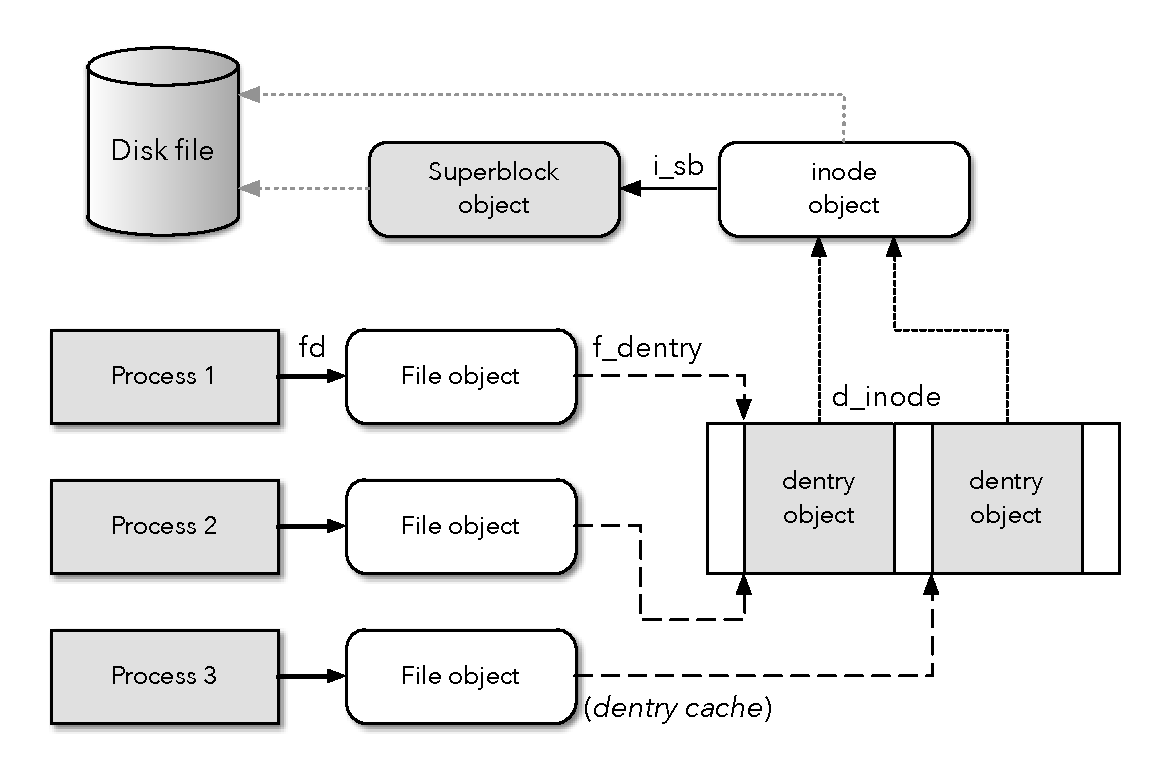
\includegraphics[width=\textwidth]{fig/vfs_objects.pdf}
  \caption{虚拟文件系统各对象关系}
  \label{fig:vfs_obj}
\end{figure}

\subsubsection{Superblock}
Superblock是整个文件系统的控制数据结构,
内存中结构的某些域在磁盘上有永久存储的映像。
Linux超级块由\struct{super\_block}表示,
其中几个重要的域包括
\struct{s\_blocksize}(文件系统块大小)、
\struct{s\_type}(文件系统类型描述子)、
\struct{s\_maxbytes}(最大文件尺寸)、
\struct{s\_dirty}(改动过的inode链表)、
\struct{s\_op}(超级块方法)、
\struct{s\_fs\_info}(对应物理文件系统超级块信息)等等。
出于效率考虑,
物理文件系统超级块\struct{s\_fs\_info}通常会在内存中缓存,
一旦出现对超级块的改动,
域\struct{s\_dirt}被置,
超级块在未来某个时候会被更新到磁盘上。

超级块的方法除了对超级块本身的操作
(\func{put\_super}、\func{write\_super})之外,
最重要的就是对inode的分配、释放、和修改
(\func{alloc\_inode}、\func{destroy\_inode}、
  \func{dirty\_inode}、\func{write\_inode})等等。
有趣的是超级块方法中没有从磁盘读入超级块的\func{get\_sb},
这其实是合逻辑的,
因为超级块的读入显然要先于超级块对象存在,
即需要一层逻辑处于超级块之外的软件完成将超级块从磁盘读入,
这一功能由\struct{filesystem}类型的\func{get\_sb}方法完成。

\subsubsection{inode}
inode对象是文件的控制块,
和文件一一对应,
磁盘文件系统的inode显然需要永久存储映像。
重要的域如下表所示:

\begin{table}[ht]
  \centering
  \begin{tabular*}{0.755\textwidth}{lll}
    \hline
    类型 & 域 & 描述\\  
    \hline
    \struct{unsigned long} & \struct{i\_ino} & inode number\\
    \struct{struct timespec} & \struct{i\_atime} & 最后访问时间\\
    \struct{struct timespec} & \struct{i\_mtime} & 最后写入时间\\
    \struct{struct timespec} & \struct{i\_ctime} & 最后修改时间\\
    \struct{unsigned long} & \struct{i\_blksize} & 文件块尺寸\\
    \struct{unsigned long} & \struct{i\_blocks} & 文件块数\\
    \struct{unsigned long} & \struct{i\_bytes} & 最后一个块的文件有效字节数\\
    \hline
  \end{tabular*}
\end{table}

\subsection{ext2/3}

\subsection{ZFS 特点}
\subsubsection{Unified Storage}
从IT管理角度,
ZFS 重大特色在于其提供统一的存储系统,
既提供文件系统服务,也提供块设备接口,
即兼具了NAS和SAN的功能,
统一存储系统使得部署和管理存储系统得到简化。

\subsubsection{Data Integrity}
ZFS 的设计最重要关注点是保护数据的完整性,
为实现这个目标,
ZFS 对所有的数据块都计算较验和,
并把较验和存储于用于寻址该数据快的快指针内,
即每个子节点的较验和存于其父节点处。

\subsubsection{Copy-On-Write}
ZFS 的另一大特色在于其数据写入方式。
和常见文件系统采用的块内直接修改不同,
ZFS 采用 COW({\em Copy-On-Write})%
\footnote{不做块内修改的思路来自{Log Structured Filesystem}}
机制写入永久存储介质。
COW 的效果就是直至修改文件系统组织树的根(即,Uberblock)之前,
所做的改动不可见并且源树不会遭到任何修改,
这期间掉电或崩溃不影响源树。
图\,\ref{fig:cow}\,展示了写入某些块的COW过程。

\begin{figure}[!ht]
  \centering
  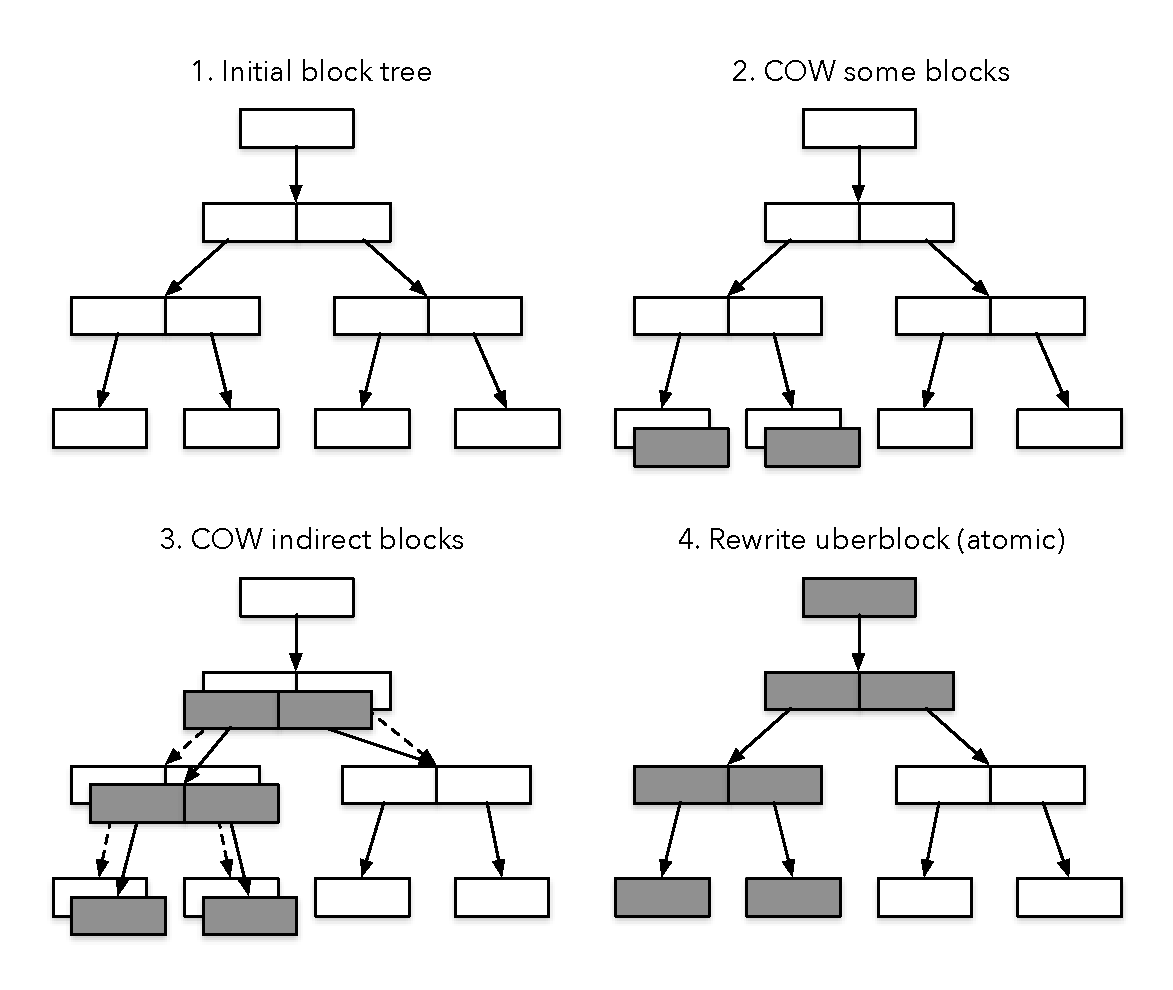
\includegraphics[width=\textwidth]{fig/zfs_cow.pdf}
  \caption{COW}\label{fig:cow}
\end{figure}

传统文件系统当掉电或系统崩溃后极容易出现\emph{文件系统}不一致。
导致不一致问题的本质原因是文件系统的数据更新涉及一系列文件系统内部结构的改动。
譬如对某个文件尾部追加一个数据块,
至少以下的几个步骤要完成:
\begin{enumerate*}[label=\itshape\alph*\upshape)]
  \item 分配一个数据块并写入该数据块;
  \item 修改维护块分配状况的数据结构,位图或B-树等;
  \item 文件的{\em inode}也需要更新,文件长度、修改时间等属性,数据块寻址数据结构。
\end{enumerate*}
这一系列改动可能部分成功部分失败,
并且不保证各部分更新的顺序。
可能有以下几种情况:
\begin{itemize}
  \item 只有数据块分配和写入成功,
    这不是问题,仅仅是刚写入的数据丢失,
    文件系统压根就不知道有这么个数据块存在过;
  \item 只有对inode的更新成功,
    这个后果就严重了,
    \begin{enumerate*}[label=\itshape\alph*\upshape)]
      \item 数据块的指针已写入,而数据未完成,于是从该指针处读出的是垃圾数据
      \item 文件系统的块管理部分未更新,而inode指出某个地址上的块有数据,
        出现文件系统不一致问题;
    \end{enumerate*}
  \item 只有块管理部分得到更新,块管理声明某个块已分配,不能挪作它用,
    但文件系统其它部分又没有使用到它,这称为空间泄漏;
  \item 块管理和inode成功更新而数据未写入,文件系统一致,但用户将得到垃圾数据;
  \item inode和数据写入而块管理未更新,文件系统不一致;
  \item 块管理和数据写入而inode未更新,空间泄漏。
\end{itemize}

传统文件系统通过{\em fsck}工具来解决不一致问题。
\begin{itemize}
  \item fsck从超级块开始,
    检查其正确性,
    如果需要从已知健全的备份超级块恢复;
  \item 而后fsck扫描所有的inode,
    数据块指针,间接快指针,根据它们判断那些块已分配,
    如果和块管理不一致,以inode为准修改块管理数据结构;
  \item fsck试图修正inode的状态,譬如文件类型等属性,
    如果发现inode无法被修正,该inode被丢弃,
    并相应修改块管理数据结构与之匹配;
  \item 修复inode和目录之间链接,
    这通过从根目录开始扫描所有的目录,计算哪些目录项链接到某个inode,
    如果数目不一致,通常修正inode中的链接数;
  \item 一旦发现有多个块指针指向同一块地址,
    如果其中有明显错误,fsck丢弃该块指针,
    否则fsck创建数据块的拷贝,使每个块指针指向自己独享的块;
  \item fsck检查块指针是否合法,譬如其是否指向硬盘分区之外的地址,
    如果块指针被发现不合法,
    fsck能做的最好处理就是从inode或间接指针中删除它;
  \item fsck也修正目录的内容,
    譬如目录``.''和``..''必须是一个目录的头两个目录项
\end{itemize}
可想而知,
fsck的全文件系统扫描机制非常低效。
现代的文件系统引入日志 ({\em journal}) 的概念,
即对文件系统改动之前,
将对更新全过程精确描述先写入存储介质,
当更新过程被意外中断重启系统或重新挂载文件系统时,
可以通过该日志知晓出了什么问题以及如何修复。
一个立刻浮现的问题是,
日志的内容可能很大,
如何保证日志本身的完整性?
答案是只能靠硬件保证。
\footnote{
  题外话,
  现代硬盘不保证多个写入请求按收到的顺序完成,
  即便使用写屏障({\em Write Barrier}) 也有可能被硬件忽略。
}
现代硬盘通常保证一次512字节写入的原子性,
于是日志写入分为两阶段,
\begin{enumerate}
  \item 日志写入,
    即先将日志开始标志和日志内容先写入,这一阶段的原子性无法保证,
    内容写入成功之后,文件系统:
  \item 将日志结束标志原子地写入磁盘
\end{enumerate}
这样一来,日志的完整与否可以由日志结束标志判定。
Linux的Ext4文件系统通过使用较验和实现对日志的一次性写入而不失完整性,
提高了日志写入的效率。
日志文件系统的缺点是任何数据写都要对磁盘操作两次。

回到ZFS,
正因为数据的COW语义,
没有就地修改的数据块,
意外断电或系统崩溃的恶果仅仅是丢失部分未写入数据,
文件系统的一致性得到保障而无需做fsck或日志回放。

\subsubsection{Snapshot \& Clone}
得益于Copy-On-Write机制,
ZFS提供高效的快照({\em Snapshot})和克隆({\em Clone})功能。
对文件系统创建快照之后,
当写入原始文件系统发生COW,
旧数据不会被回收使用,
旧的数据块树将一直存在,
部分新数据和旧数据组成一棵新树,
呈现一个新文件系统。
克隆即可写快照,
所有内容没有被修改过的数据块被共享,
写入克隆文件系统只是导致树产生分杈而不是全部复制。

ZFS文件系统可以被移入另外一个存储池中,
更进一步,
可以被发送到远程。
send命令创建一个流呈现文件系统的状态,
这个流可以呈现某个快照的所有内容,
也可以是两个快照之间的增量,
这提供了一个高效的策略,
用于譬如在HA中同步存储池或者将存储备份至其它主机。

\subsubsection{Transactional Model}
写入请求被归入某个终将写入存储池的事务组中,
事务的含义就是写入以组为原子单位,
ZFS的DMU层不允许部分成功部分失败的情形。
每一个事务组对应文件系统一个一致的状态({\em checkpoint}),
事务组完全写入磁盘后,
即一个checkpoint产生之后,
对uberblock进行一次原子写,
更新事务组号,
于是文件系统跃迁至一个新的、一致的状态上。

\subsubsection{其它}
ZFS还提供数据压缩,加密等用户需要的功能。

ZFS 另外有几个先进的实现,
\begin{description}
  \item[ARC, {\em Adaptive Replacement Cache}]\hfill\\
    ARC 是一个物理页管理算法,效率高于传统的 LRU。
    本质上说 ARC 除了考虑页的使用时间点之外还考虑页的使用频率,
    当需要回收页时,
    ARC算法有效决定从LRU还是LFU链表中选取,
    并动态、自适应地决定两条链的长度。
    除了位于内存中的缓存,
    ZFS引入了二级缓存 ({\em L2ARC}) 的概念,
    将一大部分页缓存放在SSD上免去某些页被换出后需要再次读取而操作磁盘;
  \item[ZIO pipeline]\hfill\\
    将I/O分为20道工序,
    按流水线方式处理,
    使得I/O不同阶段的工序可以在不同的CPU核上完成,
    充分利用多核CPU并行运算能力从而提高吞吐量;
  \item[Space Map]\hfill\\
    实现高效分配、释放存储设备上的块。
\end{description}

\subsubsection{缺点}
COW 的优点是集中了分散的写,
如写不同文件的数据,
又如文件的数据写伴随metadata的写\footnote{数据和元数据往往距离较远},
使它们成为线性写,
大大提高写效率。
但是这产生一个副作用,
文件相邻的块物理上可能非常分散,
造成读效率较低,
这个只能通过大内存做cache和好的缓存算法来适当抵消。

COW 另外一个缺点是会导致碎片,
在磁盘使用率超过70\%,
所有的metaslab都已创建,
其中都或多或少被填充,
文件写入将出现性能瓶颈,
IOPS下降较严重。

\subsection{ZFS组织结构}
一个存储池{\em zpool}是由虚拟设备{\em vdev}节点构成的一棵树。
位于叶端的是负责实际数据存取的物理介质,
故称为{\em phsical vdev};
其余的节点统称为{\em logical vdev},
用于表示 ZFS 的逻辑。
ZFS 藉由抽象的虚拟设备树即可实现不同的Raid级别。

\begin{figure}[ht]
  \centering
  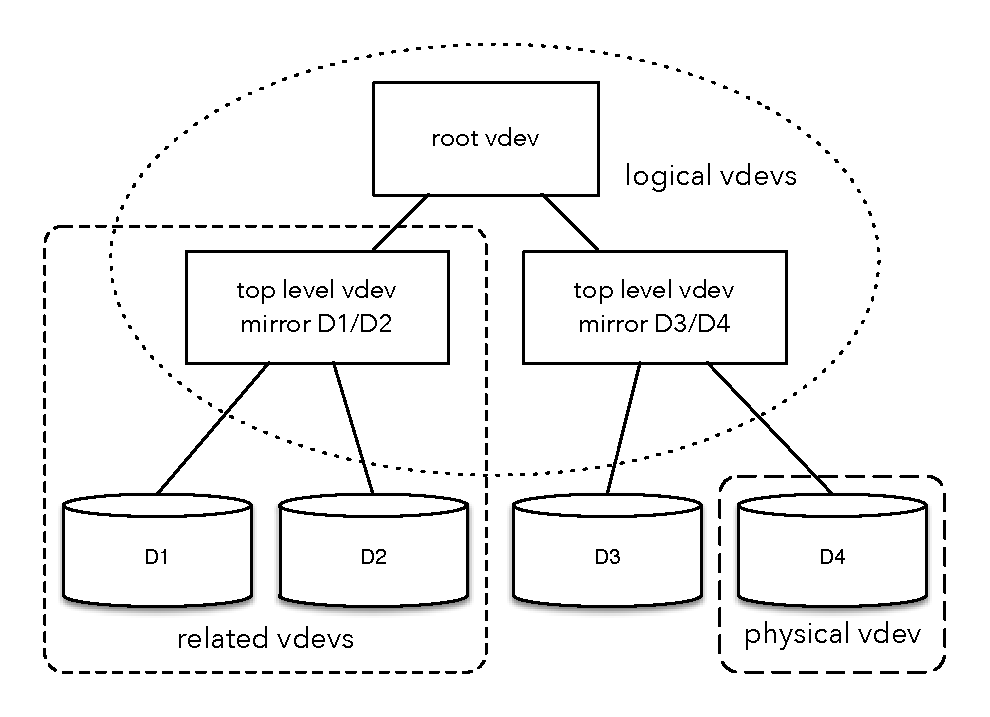
\includegraphics[width=\textwidth]{fig/zfs_architecture.pdf}
  \caption{ZFS架构}\label{fig:arch}
\end{figure}

图\,\ref{fig:arch}\,所表示的存储池结构由如下命令创建,
第二个 mirror 关键字表示将指定新的顶层虚拟设备。
数据通过这两个镜像以动态方式进行条带化,
并会相应地在每个磁盘之间创建冗余数据。
\begin{lstlisting}{lanuage=Bash}
# zpool create tank mirror D1 D2 mirror D3 D4
\end{lstlisting}

\subsection{ZFS代码模块}
从设计实现的角度看,
ZFS 分为 7 个相对独立模块,
模块的简称贯穿整个ZFS文件系统的代码及文档之中。

\begin{description}
  \item[SPL, {\em Storage Pool Allocator}\,:]
    负责存储池一级的操作,如创建,销毁,修改属性等;
  \item[DMU, {\em Data Management Layer}\,:]
    完成将数据块组织为对象,如文件、目录等,
    并且将对象组织为对象集,如文件系统、文件系统快照等;
  \item[DSL, {\em Dataset and Snapshot Layer}:]
    管理对象集属性以及各对象集之间逻辑关系
  \item[ZAP, {\em ZFS Attribute Processor}\,:]
    位于 DMU 层之上,
    操作称为 ZAP 的对象,
    ZAP 对象用于描述如文件系统、存储池等对象集的属性;
  \item[ZPL, {\em ZFS Posix Layer}\,:]
    将 ZFS 的对象、对象集以 Posix 标准的方式呈现,
    提供 POSIX 标准方式的文件操作,如 open、read、write;
  \item[ZIL, {\em ZFS Intent Log}\,:]
    ZIL 保存来自系统调用的写操作的纪录,
    描述写操作本身的数据量比为维护文件系统一致性%
    而引发的一连串写要小多了。
    ZIL 用于当系统崩溃或意外掉电时回放该事务,
    可找回部分数据。
    启动一个 DMU 事务同时会启动一个 ZIL 事务,
    并在 {\em fsync}%
    \footnote{{\em fsync}的语义就要求写入被从内存中刷到永久存储介质上}
    时被写入永久存储设备。
    但此时文件系统的checkpoint还未真正完成,
    如果此时掉电或系统崩溃,
    文件系统仍处于之前一个一致的checkpoint,
    这种情况就可以通过对ZIL的{\em reclaim}来追回数据。
    当该 DMU 事务成功完成之后,
    因为一个一致的checkpoint已经产生,
    之前写操作的 ZIL 可以丢弃;
    通常采用一个快速 SSD 专门用于 ZIL 存储设备提高效率;
  \item[ZVOL, {ZFS Volumes}\,:]
    提供一种创建、使用逻辑卷的机制,
    将 ZFS 卷以块设备的形式,通过诸如iSCSI接口呈现给用户。
\end{description}


\subsection{ZFS磁盘格式}
\subsubsection{vdev label}
访问文件总是从物理介质的某个已知的固定位置读取文件系统的元数据开始,
传统文件系统的元数据称为超级块,
ZFS的术语就是{\em vdev label}和{\em Uberblock}。
ZFS在磁盘的起始和结尾存储了四份vdev label。
对vdev label的更新是唯一不遵循COW原则的点。
ZFS采用两阶段提交的方法保证完整性,
具体说就是先更新偶数号的label再到奇数号的,
这样万一在更新某个label时发生掉电仍然有健全的label可用。
vdev label的结构及其在磁盘上的分布如图\,\ref{fig:vlabel}\,所示。

\begin{figure}[ht]
  \centering
  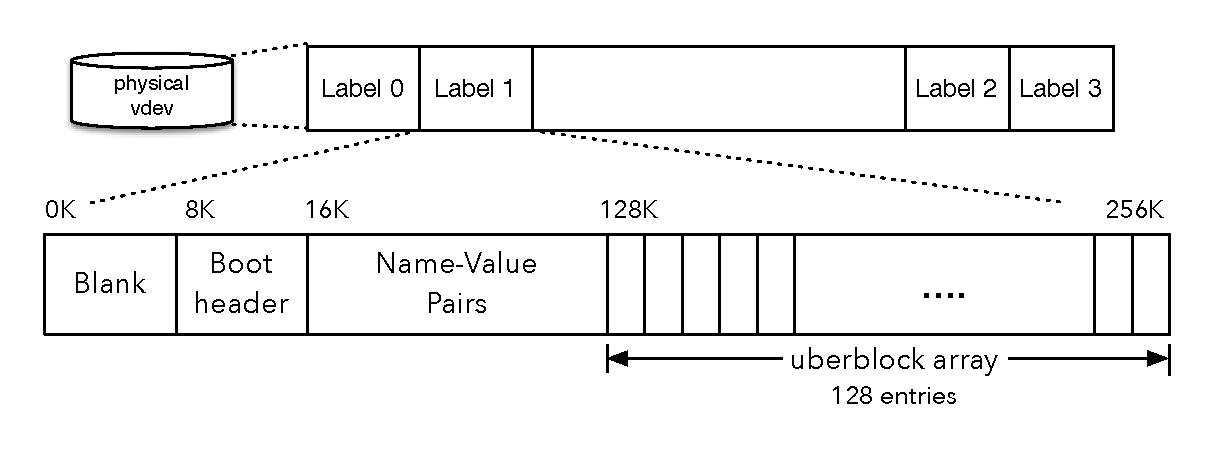
\includegraphics[width=\textwidth]{fig/zfs_vdev_label.pdf}
  \caption{Vdev Label}\label{fig:vlabel}
\end{figure}

\subsubsection{块指针}
除位于固定位置的元数据vdev label外,
所有其它数据位置都是动态分配的,
访问它们都必须通过块指针。
确切地说,
块指针是一个数据块的描述子,
除了记载块在磁盘上的逻辑地址以外,
还有较验和,块类型等域,
块指针结构如\,\ref{fig:blkptr}\,所示。

\begin{figure}[ht]
  \centering
  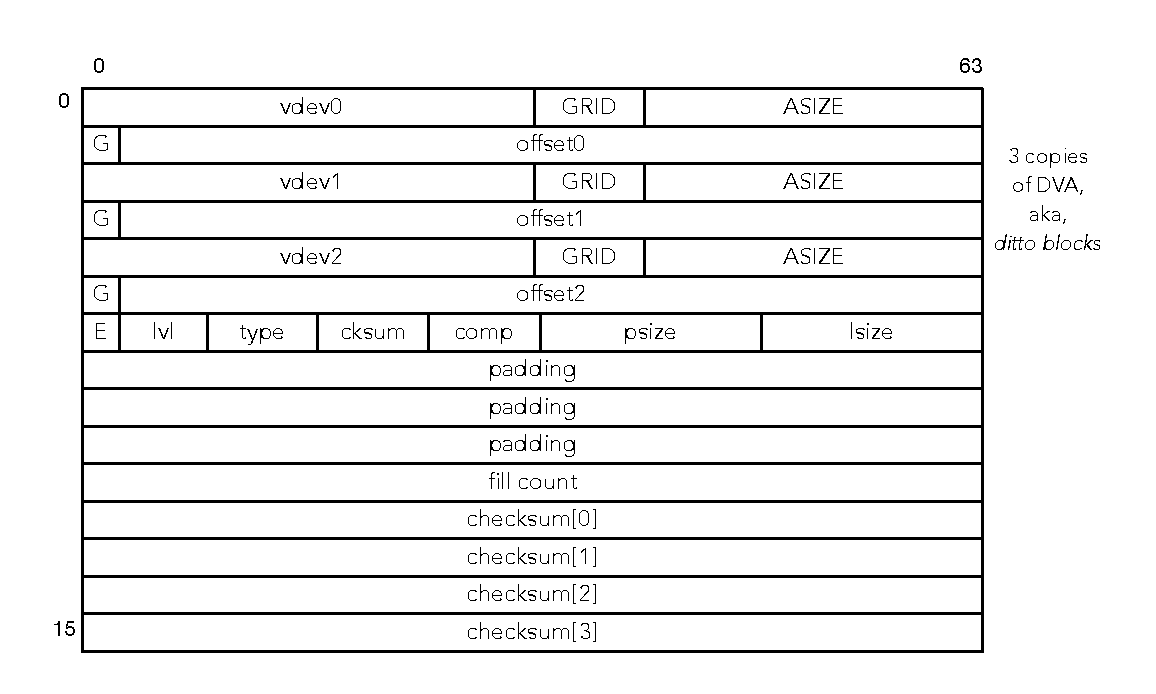
\includegraphics[width=\textwidth]{fig/zfs_blkptr.pdf}
  \caption{Vdev Label}\label{fig:blkptr}
\end{figure}

值得一提的是一个数据块在磁盘上最多可以有三个备份,
ZFS术语称为{\em ditto blocks}。
Uberblock结构有一个\verb|ub_rootbp|域,
游历文件系统数据块就从那里开始。

\subsubsection{对象}
若干数据块以一定方式组织成为对象({\em Object}),
如面向用户的POSIX文件对象(\verb|DMU_OT_PLA-IN_FILE_CONTENTS|)%
和POSIX目录对象(\verb|DMU_OT_DIRECTORY_CONTENTS|),
还有维护ZFS内部逻辑用的\verb|DMU_OT_SPACE_MAP|、
\verb|DMU_OT_DNODE|等对象。

对象的描述子称为{\em dnode},
磁盘上结构为\verb|dnode_phys_t|。
粗略地,
可以把 \verb|dnode_phys_t| 看作 一个模版,
各种类型的对象是这个模版的不同实例,
一个dnode描述相关的数据块如何被组织成该类型的对象。
譬如文件对象描述其所有数据块在磁盘中的分布;
又如目录对象描述如何在该目录下根据文件名检索到对应的文件对象。
dnode类型定义如代码段\,\ref{src:dnode}\,所示。
\inputclisting{zfs_src/dnode.h}
              {ZFS对象}{src:dnode}
一个dnode只包含一个块指针,
ZFS数据块最大尺寸128K,
文件数据超过这一尺寸就需要引入间接块,
ZFS支持最多6级间接寻址,
除第一级间接块尺寸为16K可容纳$2^7$个块指针,
其余均可达到块最大限制128K可容纳$2^{10}$个块指针,
可计算出一个对象的最大尺寸为$2^{7 + 7 + 10 \times 5} = 2^{64}$字节。
图\,\ref{fig:dn_ind}\,演示了一个三级间接寻址。
\begin{figure}[!ht]
  \centering
  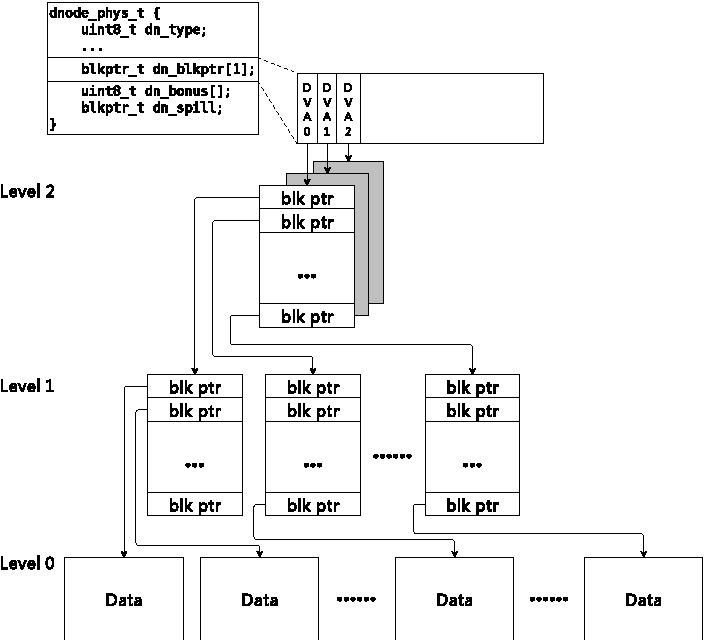
\includegraphics[width=.8\textwidth]{fig/zfs_ind_blkptr.pdf}
  \caption{三级间接寻址}\label{fig:dn_ind}
\end{figure}
              
\subsubsection{对象集}
除了负责将数据块组织成对象,
DMU这一层也管理由多个对象组成的对象集({\em Object Set}。)
换句话说是对象集的数据就是一个个dnode。
对象集有三种,
分别是\verb|DMU_OST_META|、\verb|DMU_OST_ZFS|及\verb|DMU_OST_ZVOL|。
磁盘上描述对象集的数据结构{\em objse\_phys\_t}
定义如代码段\,\ref{src:objset}\,。
\newpage
\inputclisting{zfs_src/objset.h}
              {ZFS对象集}{src:objset}

\begin{figure}[!ht]
  \centering
  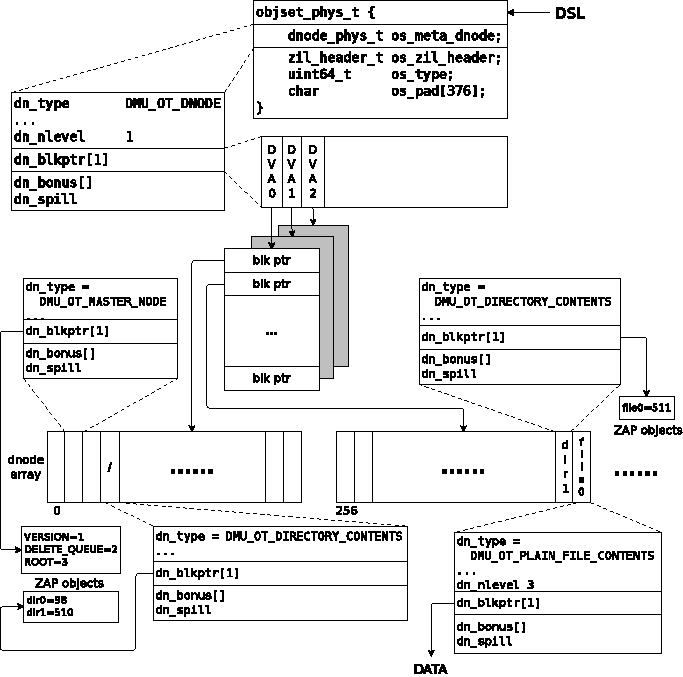
\includegraphics[width=\textwidth]{fig/zfs_objset.pdf}
  \caption{对象集内部组织结构}\label{fig:zfs_objset}
\end{figure}

图\,\ref{fig:zfs_objset}\,示例一个由文件系统对象集定位到指定对象的过程。
从中可以看到,
对象集作为检索对象的起始点,
其结构包含一个dnode类型的域,其类型为\verb|DMU_OT_DNODE|,
换句话说,
该dnode域描述的数据类型为dnode。
另外值得注意的是它的\verb|dn_nlevel|域为1,
说明其描述的dnode寻址树有一级间接寻址。


一个dnode尺寸为512字节,
由上面的计算可知,
一个对象集最多可以容纳$2^{64} / 2^{9} = 2^{55}$个对象。
对象集的数据\,---\,dnode以数组形式存储索引,
每个对象在dnode array中有一个唯一索引号。
索引号为1的dnode有特殊用途,
视对象集的类型而定。
对文件系统类型来说,
该特殊dnode所描述的对象为\verb|DMU_OT_MASTER_NODE|类型,
即一种ZAP对象,
其数据块中存储的信息包括了根目录对象在数组中的索引号,
图中那个``\verb|ROOT=3|''项。
从这里开始就可以遍历访问整个文件系统。
注意到目录类型的对象存储的都是 name-value 对,
value 部分就是对应该名字的dnode在数组中的索引
图中接地的那部分就进入上一节描述的游历一个对象的所有数据块过程。

\subsubsection{DSL}

\begin{figure}[!ht]
  \centering
  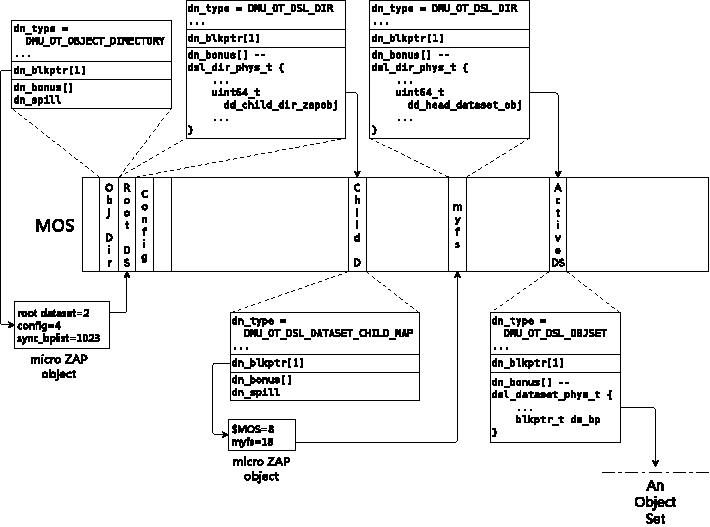
\includegraphics[width=.95\textwidth]{fig/zfs_dsl.pdf}
  \caption{MOS dnode数组结构}\label{fig:mos}
\end{figure}

如何检索到到一个指定的对象集由DSL层负责。
DSL层在磁盘上也呈现为一个对象集,
也就是说它所存储处理的数据也是对象描述子\,--dnode,
这一层对象集的类型为\verb|DMU_OST_META|,
即所谓MOS({\em Meta Object Set}),
MOS也是一个dnode数组。
作为目录项,
MOS中很多项的块指针指向的ZAP对象中存储的是另外某些项在数组中索引的位置,
如图\,\ref{fig:mos}\,中的{\em Object Directory}项描述的数据对象中的%
``root dataset=2'',
又如{\em Child Directory}项数据中的%
``myfs=18''。

在刚引入dnode概念的时候有一个细节没有提及,
就是\verb|dn_bonus|域,
该域有时被用来存储比较小的数据避免分配一个大块。
\footnote{{\tt dmu\_bonus\_hold}函数是个好例子。}
例如图\,\ref{fig:mos}\,中,
文件系统dnode为存储管理活跃的数据集的dnode在MOS的索引没有动用块指针那套机制,
而是在\verb|dn_bonus|中存储\verb|dsl_dir_phys_t|的结构,
这个结构的\verb|dd_head_dataset_obj|域就是当前活跃数据集的dnode在MOS中的索引值;
又如描述活跃对象集的dnode的\verb|dn_bonus|域中存储的是%
\verb|dsl_dataset_phys_t|结构,
通过这个结构的\verb|ds_dp|域指向的数据块即可进入由对象集向对象的检索阶段。
无法将下一层的\verb|objset_phys_t|也嵌入到\verb|dn_bonus|中因为%
\verb|objset_phys_t|本身含有一个dnode结构,
不得已只好开一个块来存储它。

MOS如何寻址得到呢?
答案就是Uberblock。
图\,\ref{fig:uber}\,示意如何完成在磁盘上寻址MOS。
如前所述,
vdev label和uberblock作为整个检索树的根,
必须位于磁盘的固定位置为软件层预先知晓。
\begin{figure}[!hb]
  \centering
  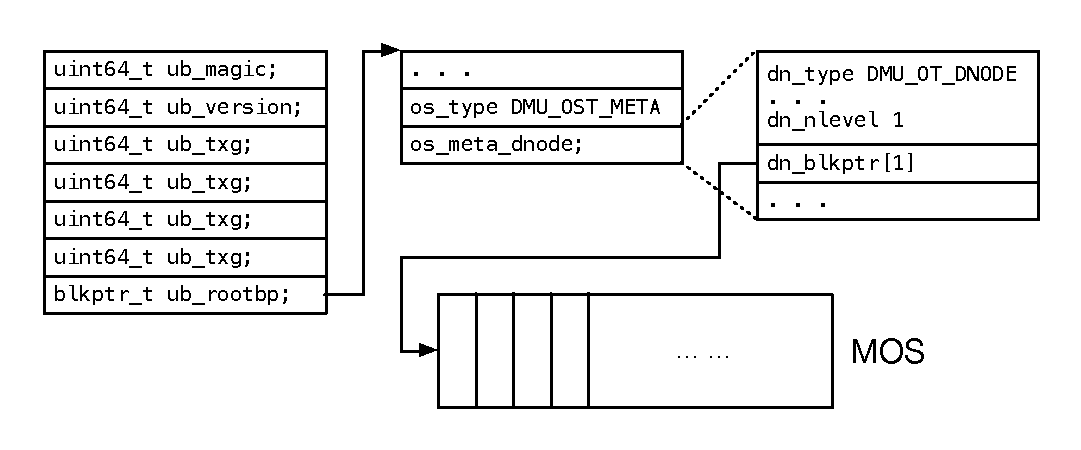
\includegraphics[width=.95\textwidth]{fig/zfs_uber_to_mos.pdf}
  \caption{由Uberblock到MOS}\label{fig:uber}
\end{figure}

\subsection{ZFS块管理---{\em Space Map}}
\subsubsection{位图}
传统的块管理一般使用位图,
思路简单,
一个位表示一个块,
一个字节可以表示8个块,
如果采用4K块大小,
在1T的磁盘上,
需要32M字节的位图,
1PB就需要32G字节,
空间使用和扫描位图的时间开销开始不可接受。
为优化扫描效率,
一个看似可行的方案是将位图分区,
每一个区维护一个整数纪录该区的空闲块数量,
这避免了每一次都扫描整个大位图而只需扫描一个小分区,
譬如1PB的大位图可以分成1M个区。
但这方案仍然有个大问题,
不但分配块需要读写位图,
释放块一样需要。
譬如在1PB的文件系统中删除一个4GB的文件,
需要释放1M个块,
也就是说修改1M个位,
如果运气不好,
上述的1M个位图分区都要被访问到,
这开销太大。
另外当内存容纳不下整个位图,
随机地分配和释放块伴随的位图更新操作将导致大量的磁盘写入。

\subsubsection{B-树}
B-树方案就是在磁盘上存储一棵以{\em extent}%
(即一个起始地址和从那开始的长度)为key的B-树,
这解决一个问题,
就是一次分配或释放一个大连续块组,
只做少数的几个磁盘写入即可更新块管理数据结构,
比位图的一一对应效率高了很多。
大量随机分配释放小块使得在树的各个节点都要更新,
也没有大的extent,
都是描述小extent的节点,
巨额开销仍无法避免。

\subsubsection{延迟释放}
对上述两种数据结构可以做一个优化就是延迟释放,
以期未来某个时候需要分配一个新块的时候直接交付,
直到释放块的数量达到一个阈值对要释放的块地址进行排序,
按顺序更新磁盘上的位图或树,
大大降低了开销。

\subsubsection{Space Map}
ZFS则创新地采用类似log结构的方式存储磁盘块使用信息,
称为{\em Space Map}。Jeff Bonwick在他的博客中提到:

\begin{quotation}
  Recall that log-structured filesystems long  ago posed this question: what if,
  instead of periodically folding a transaction log back into the filesystem, we
  made the transaction log be the filesystem?

  Well, the  same question could  be asked of our  deferred free list:  what if,
  instead of folding it into a bitmap  or B-tree, we made the deferred free list
  be the free space representation?
\end{quotation}

ZFS的确就是这么做的。
ZFS把物理设备划分为一百多个slab,
每个slab有一个块管理数据结构 space map,
当分配或释放某个extent时,
就往space map中追加一条log记录下这一事件,
因为它总是以追加方式记录,
并且由于采用了延迟释放,
随机释放和连续释放效率一样,

另外一个美妙的地方在于当加载一个存储池时,
space map会在内存中表现为一棵按磁盘上地址排序的AVL树,
其节点就是所有空闲块的extent。
这样常常可以将多条log抵消,
或合并为一个节点,
使得树并不很大,
在分配和释放过程中AVL也时不时合并和拆分节点,
再将space map写回磁盘去也不会太大。
极端的例子就是加载一个全满和全空的在内存中AVL树结构一样,
就一个节点。


\subsection{ZFS I/O流水线}
\subsubsection{zfs\_write}
\begin{figure}[!h]
  \centering
  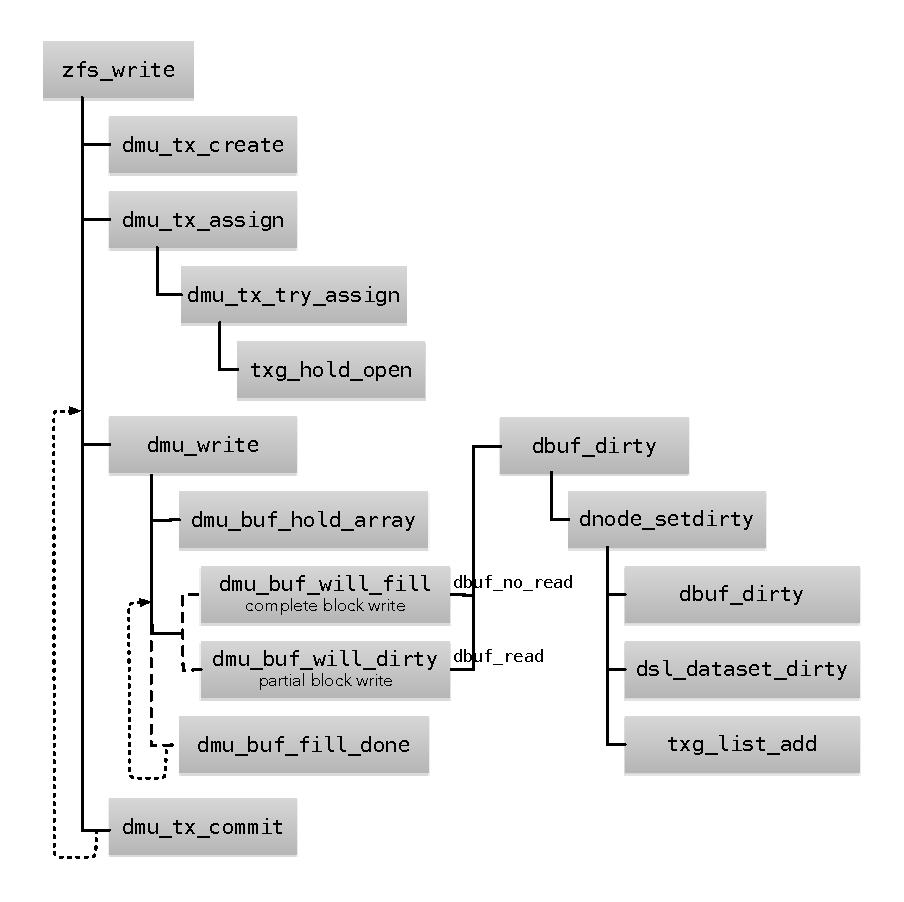
\includegraphics[scale=0.85]{fig/zfs_write.pdf}
  \caption{ZFS 写请求处理流程}\label{fig:zfs_write}
\end{figure}

系统调用和ZFS在写操作方面的交界点在\verb|zfs_write|函数,
此函数从用户空间获取数据并传给DMU层完成写入。
如果用户数据量大就需要将数据分成多个块,
为每一个块开启一个事务,
将事务加入事务组,
写数据块将触发一系列上游节点数据的更新,
将所有的更新都加入同一事务组。
大致调用链如图\,\ref{fig:zfs_write}\,所示。
最后一步提交事务,
负责处理事务组的线程被唤醒,
将事务取下,
完成对物理设备的写入工作。

\subsubsection{事务组}
一个事务组经历三个状态,
\begin{itemize}
  \item open: 新创建事务组即处于open状态,
    对内存中数据结构的更新在这状态中完成
  \item quiescing: 一个缓冲状态,
    这个状态的目的是等待所有组内的事务被提交,
    即过了此阶段,
    不会再有新的事务进入这个事务组,
    一般处于这个状态的事件都很短暂
  \item syncing: 在这个状态,
    将内存中更新写入永久存储介质
\end{itemize}

当创建或加载一个存储池时,
两个事务组线程被创建,
一个负责quiesce,
另一个负责sync。

负责sync的线程被唤醒之后调用\verb|spa_sync|函数,
从这个点到最后触发zio的调用链如图\,\ref{fig:spa_sync}\,所示。
\verb|dsl_pool_sync| 中 \verb|dsl_dataset_sync| 被调用了两次,
每一次都阻塞等带 I/O 返回,
在这一步 I/O 失败被认为是很严重事件,
kernel panic。

\begin{figure}[!ht]
  \centering
  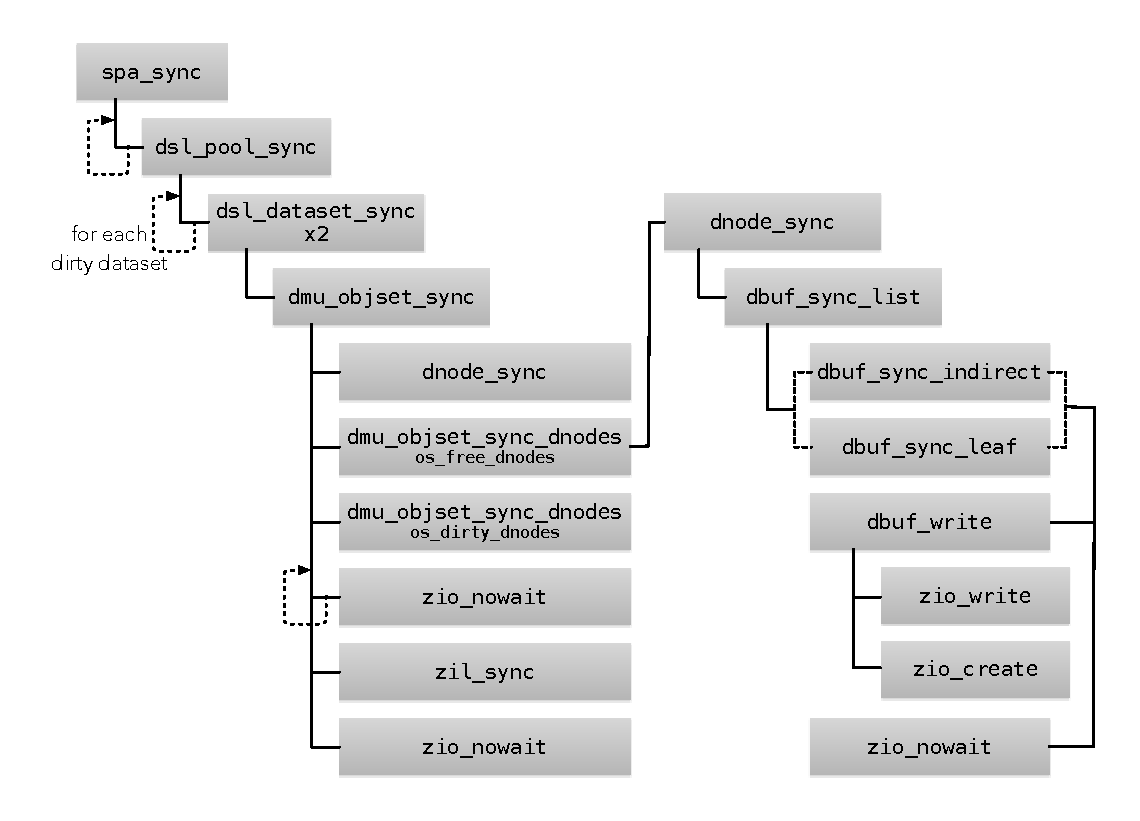
\includegraphics[width=\textwidth]{fig/zfs_spa_sync.pdf}
  \caption{sync到zio的流程}\label{fig:spa_sync}
\end{figure}

\verb|dbuf_sync_leaf|将数据异步地写出。
为了支持 COW,
数据块更新几次,
间接块必须相应更新几次。
\verb|dbuf_sync_indirect|函数对间接块进行读、修改其内容,
创建 ZIO 而后执行写出。

\subsubsection{I/O流水线}
执行 ZIO 的线程不是将整个I/O过程从头至尾执行,
为了提高吞吐率,
充分利用多核特性,
I/O被分为多道工序,
以优化方式分配给流水线上的工作线程。

I/O操作分为五类,
\begin{enumerate*}[label=\itshape\arabic*\upshape)]
  \item Read
  \item Write
  \item Free
  \item Claim
  \item Ioctl
\end{enumerate*}
这五类操作由不同的工序按指定顺序组合而成。

ZIO流水线的核心函数是\verb|zio_execute|。
和工厂流水线上工人一人只负责某几道确定工序不同,
ZIO 的线程可以负责任意工序,
一个线程完成某道工序之后有两种可能,
如果工序例程调用\verb|zio_taskq_dispatch|将
将半成品挂到某个队列上返回\verb|ZIO_PIPELINE_STOP|,
\verb|zio_execute|停止执行,返回,
之后工序交给谁处理由上一层逻辑按优化方式决定(当然可能还是同一个线程);%
\footnote{这里可能有优化余地,
  即让线程自己根据优化逻辑决定是挂出半成品还是自己继续处理}
否则例程会返回\verb|ZIO_PIPELINE_CONTINUE|,
当前线程在\verb|zio_execute|中继续调用下一道工序例程。

Write:
举例来说,
写操作的流水线定义如下:

\begin{lstlisting}{lanuage=C}
#define ZIO_WRITE_COMMON_STAGES		\
        (ZIO_INTERLOCK_STAGES	|	\
         ZIO_VDEV_IO_STAGES	|	\
         ZIO_STAGE_ISSUE_ASYNC	|	\
         ZIO_STAGE_CHECKSUM_GENERATE)
\end{lstlisting}

根据定义:

\begin{lstlisting}{lanuage=C}
 ZIO_STAGE_READY		= 1 << 16,	/* RWFCI */
 ZIO_STAGE_DONE			= 1 << 21,	/* RWFCI */
 ZIO_STAGE_VDEV_IO_START	= 1 << 17,	/* RWF-I */
 ZIO_STAGE_VDEV_IO_DONE		= 1 << 18,	/* RWF-- */
 ZIO_STAGE_VDEV_IO_ASSESS	= 1 << 19,	/* RWF-I */
 ZIO_STAGE_ISSUE_ASYNC		= 1 << 3,	/* RWF-- */
 ZIO_STAGE_CHECKSUM_GENERATE	= 1 << 5,	/* -W--- */
\end{lstlisting}

各道工序的例程在\verb|zio_pipeline|中定义:
\begin{lstlisting}{language=C}
static zio_pipe_stage_t *zio_pipeline[] = {
	NULL,
	zio_read_bp_init,
	zio_free_bp_init,
	zio_issue_async,
	zio_write_bp_init,
	zio_checksum_generate,
	zio_nop_write,
	zio_ddt_read_start,
	zio_ddt_read_done,
	zio_ddt_write,
	zio_ddt_free,
	zio_gang_assemble,
	zio_gang_issue,
	zio_dva_allocate,
	zio_dva_free,
	zio_dva_claim,
	zio_ready,
	zio_vdev_io_start,
	zio_vdev_io_done,
	zio_vdev_io_assess,
	zio_checksum_verify,
	zio_done
};
\end{lstlisting}

也就是说要完成\verb|zio_write|,
以下流水线上函数将被依次调用:
\begin{lstlisting}{lanuage=C}
 zio_issue_async,
 zio_checksum_generate,
 zio_ready,
 zio_vdev_io_start,
 zio_vdev_io_done,
 zio_vdev_io_assess,
 zio_done
\end{lstlisting}

\verb|zio_issue_async|函数将zio挂如一个taskq线程的队列,
告知\verb|zio_execute|立即返回,
taskq线程完成余下工作。

\verb|zio_checksum_generate|函数生成较验和之后返回
\verb|ZIO_PIPELINE_CONTINUE|,
于是该taskq线程继续下一道工序,即\verb|zio_ready|。

\verb|zio_ready|一开始调用\verb|zio_wait_for_children|,
如果zio有gang或者ddt类型的子zio,
\verb|zio_wait_for_children|将工序移至下一道,
但状态设为{\em stall}并返回stop,
使得\verb|zio_execute|直接返回,
zio的工序暂停,
直至所有子zio都到达\verb|READY|阶段以后才能继续执行。
\verb|zio_ready|将调用\verb|zio_notify_parent|,
\verb|zio_notify_parent|又调用\verb|zio_execute|%
继续父zio刚才暂停的工序,
当然并非一定是该线程完成,
依然可能是将zio挂到某个taskq的队列中就返回。

下一道工序是\verb|zio_vdev_io_start|,
它负责为物理I/O做准备。
如果该zio的vdev是物理设备,
调用\verb|vdev_queue_io|将zio挂入vdev的队列,
返回\verb|STOP|;
否则直接调用该设备的\verb|vdev_op_io_start|%
(可能是mirro,或者Raid等等)
方法将zio逐层下传至物理设备。
这一道工序总是返回\verb|STOP|。

\verb|zio_vdev_op_io_done|主要就是错误处理,
之后就是收尾的两道工序。

\subsubsection{ARC及L2ARC}
LRU:
考虑如下场景,
当程序一次性地读入大量数据(常见的例如:\verb|grep -nr|),
那些数据块轻易填满cache,
挤出大量的页,
但它们仅仅被使用一次,
滞留在cache中毫无益处。
那些被频繁使用的页却被无谓地换出。
另外一方面,
单单考虑页面访问频度的策略也有其缺陷,
ARC的思路是同时采纳两种策略,
并且自适应地在二者间做权衡。

ARC:
ARC维护两个先进先出的页面队列,
分别存放按MRU和MFU策略处理的页描述子。
MRU和MFU还各自有一个ghost队列。
页面第一次被读入并缓存时,
插入MRU队列头部,
当它第二次被访问就移入MFU队列,
在MFU队列中再次被访问则会移到队列头。
当cache够用时,
两个ghost队列都为空,
MFU和MRU各自扩张到最大限度。
如图\,\ref{fig:zfs_arc0}\,所示。

\begin{figure}[!h]
  \centering
  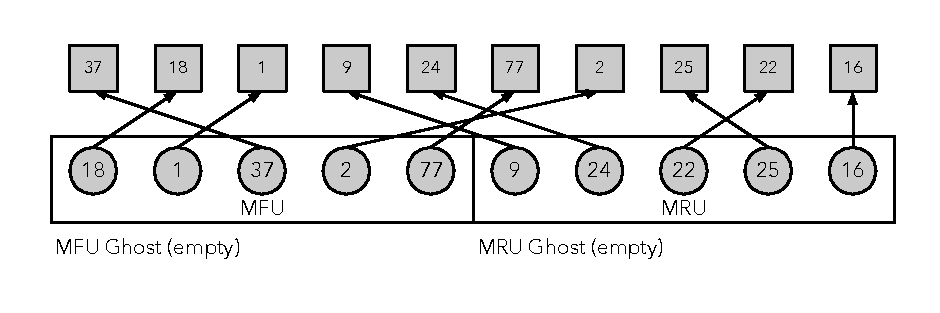
\includegraphics[width=\textwidth]{fig/zfs_arc0.pdf}
  \caption{MSU和MRU}\label{fig:zfs_arc0}
\end{figure}

\begin{figure}[!ht]
  \centering
  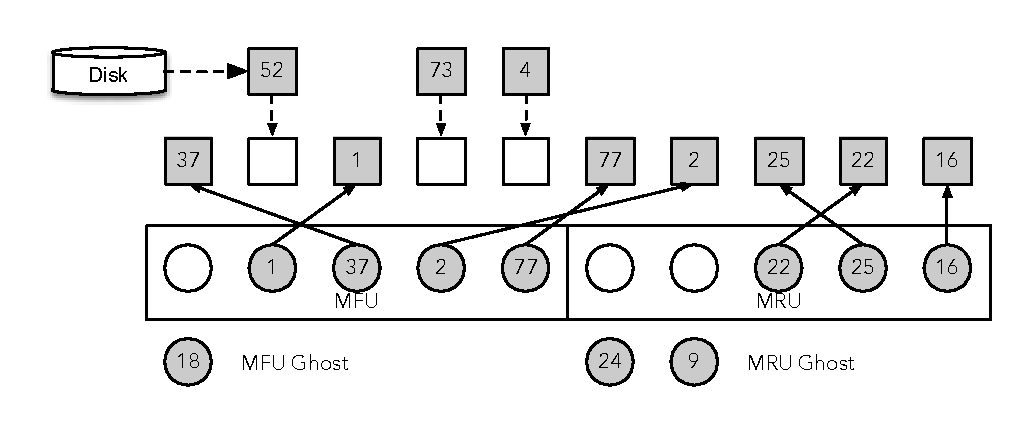
\includegraphics[width=\textwidth]{fig/zfs_arc1.pdf}
  \caption{Evicted to Ghost Lists}\label{fig:zfs_arc1}
\end{figure}

内存紧张以后,
再从磁盘读入新页将触发cache中某些页面被清除({\em evict}),
这时将该页面的描述子插入其所属页缓存类的ghost队列头,
即虽然磁盘数据块已经不在内存中,
其引用依然保留。
当然ghost队列越来越长到达最大限度以后,
页面的描述子将被依次序删除,
对应磁盘数据块的引用彻底消失。
图\,\ref{fig:zfs_arc1}\,演示了页面被evict的场景。

当已换出数据块再次被从磁盘读取,
如果发现其引用仍位于某个的ghost队列中,
这透露的一个信息是该类页缓存的miss率较高,
需要增加该类页缓存的额度,
当然同时减少另外一方的额度,
图\,\ref{fig:zfs_arc2}\,演示了这一过程。

\begin{figure}[!ht]
  \centering
  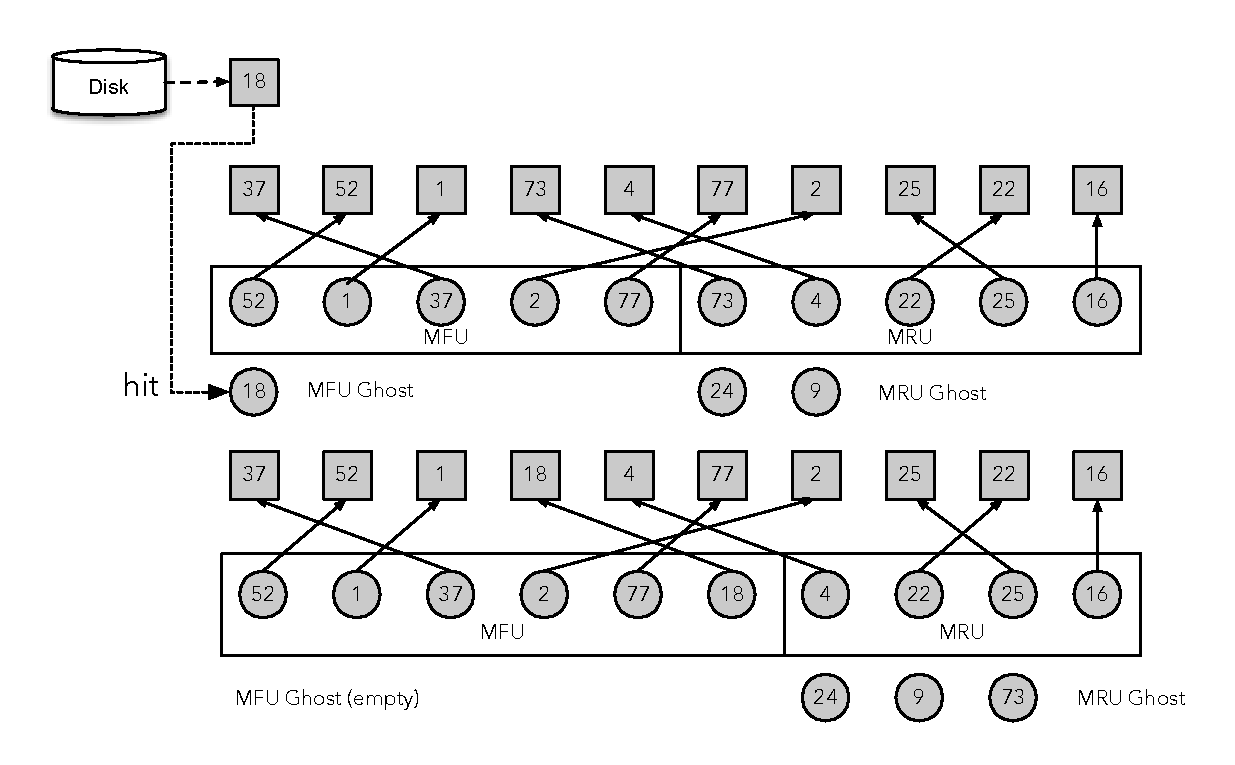
\includegraphics[width=\textwidth]{fig/zfs_arc2.pdf}
  \caption{Expand MFU and Shrink MRU}\label{fig:zfs_arc2}
\end{figure} 

两类页缓存策略采用相同的逻辑,
两种策略自适应地趋向符合work load的页使用需求。
仍然考虑之前的场景,
一次性读入大量数据导致MRU的ghost队列很长,
但它们再没有被命中过,
如果有其它的应用%
\footnote{譬如数据库在某些时候会反复执行相同的查询}%
使得MFU的ghost队列总是命中,
于是MFU的页缓存队列越来越长而MRU的页缓存队列越来越短,
逐渐达到平衡,
页面的换出策略得到优化。

ZFS对ARC的实现与源算法有些小区别。
\begin{itemize}
  \item ZFS 的缓存容量根据当前可用内存动态可变;
  \item ZFS 支持多种不同块尺寸;
  \item ZFS 支持把一个页锁在内存中,
    在清除页时需要扫一下队列找最老的可清除的页。
\end{itemize}

L2ARC:
可以让ZFS使用SSD作为二级页缓存设备,
即所谓{\em L2ARC},
它使用了一个\verb|l2arc_only|队列维护只在SSD上的页缓存。
其主要算法和ARC完全一致。
一个自然的想法使当ARC需要清除页面时,
自动地清到SSD上。
但这样将导致一些严重问题,
其一是当有一个大数据读将一次刷出大量页面到SSD上,
其二是当应用程序开辟大量内存是,
ARC需要被缩减,这时又可能导致一次性大量页面刷出。
ZFS解决方法是用一个线程\verb|l2arc_feed_thread|扫描两个缓存队列,
将最近可能要清除出去的页组到一个8M的缓冲区,
之后由另一个\verb|write_hand|线程一次性写出,
这适当降低了突发大量写的危害。


\subsubsection{Solaris fd space}
随着进程打开关闭文件,
内核时不时分配释放fd,
fd空间就会出现很多空洞。
由于历史原因,
打开文件分配fd时总是从当前可用的fd中找最小的那一个,
要快速地从中找出第一个可用的fd是一个挑战。
显然进程的fd空间[0\dots {\sc max\_fd}]可看作一棵完全二叉检索树的中序遍历,
找最小fd的过程可看作遍历二叉树在其中找一个最小的空闲节点。
方法是每个节点维护以该节点包括它子集的右子树中已分配的fd数,
通过判断当前树是否完全和右子树已分配节点数可以决定搜寻方向。
巧妙地利用二进制数的性质可以快速计算父子以及当树完全时某子树的节点数。
这样由[0\dots {\sc max\_fd}]数组表示完全二叉检索树有以下一系列属性:

\begin{enumerate}
\item 树中节点的最低被置位的位置指示该节点位于树中的第几层,
  譬如x1位于最底层 ,
  x10节点位于树的第一层,
  并且同一层的节点值从左向右递增;
  
\item 节点的右子树的节点包括它本身的个数($csize$)
  等于将该节点值仅保留最低被置位所得的值,
  譬如x10右子树的所有节点数$csize(\text{x10})$为2;
  
\item 节点$n$的最近左祖先(即$n$位于它的右子树中)
  $lparent$等于清除该节点的最低被置位,
  因为$lparent(n)$是清除最低被置位,
  而$csize(n)$是清除除最低被置位外的所有位,
  所以$lparent(n) = n - csize(n)$;
  
\item 最近的右祖先$rparent(n) = n + csize(n)$

\item 任意内部节点,
  子和父值之差为$csize(parent) / 2$。
\end{enumerate}

根据:
\begin{eqnarray}
  n &=& \textit{xxxx10}\dots{\it 0}\\
  n - 1 &=& \textit{xxxx01}\dots{\it 1}\\
  n \;\&\; (n - 1) &=& \textit{xxxx00}\dots{\it 0}\\
  n \,\mid\, (n - 1) &=& \textit{xxxx11}\dots{\it 1}\\
  n \,\XOR\, (n - 1) &=& \textit{000011}\dots{\it 1}
\end{eqnarray}

可以快速地计算出:
\begin{eqnarray}
  csize(n) &=& (n - 1) \,\XOR\, (n \,\mid\, (n - 1))\\
  lparent(n) &=& n \;\&\; (n - 1)\\
  rparent(n) &=& (n \,\mid\, (n − 1)) + 1
\end{eqnarray}

考虑到fd从0开始,
公式中变量值由$n$变为$n' = n - 1$,
并且计算出的fd值要减去1,
于是真正实现中使用的公式为:

\begin{eqnarray}
  csize(n) &=& n \,\XOR\, (n \,\mid\, (n + 1))\\
  lparent(n) &=& n \;\&\; (n + 1) - 1\\
  rparent(n) &=& (n \,\mid\, (n + 1))
\end{eqnarray}

具体到代码实现,
\struct{proc\_t.p\_user.u\_finfo.fi\_list}就是进程的fd空间数组,
数组元素类型为\struct{uf\_entry},
数组元素逻辑上看作二叉树中的一个节点,
数组索引$n$就是节点值,
域\struct{uf\_alloc}被用于存储节点$n$当前右子树(包括它自己)的总节点数,
如果\struct{uf\_alloc}不等于$csize(n)$,
说明在它的右子树里至少有一个fd可用。

函数\func{fd\_find}接受一个minfd参数,
完成搜寻$\ge\,$minfd的fd中最小的那一个。
打开文件时通常传入0作为minfd参数。
搜寻的过程如下:
\begin{enumerate}
\item 从以minfd为根的树找起,
  计算$csize(minfd)$,
  和\struct{fi\_list[minfd].uf\_alloc}比较,
  如果不等,
  说明在minfd的右子树下可以找到一个空闲的fd,这一步结束;
  否则上溯到minfd的右祖先,
  继续这一步直至找到某个节点fd满足$csize(fd)$不等于
  \struct{fi\_list[fd].uf\_alloc};
\item 从上一步得到的节点为根,
  开始搜寻树中最小的空闲fd,
  查左子树而后右子树。
\end{enumerate}

\inputclisting{snippet/fio.c}
              {fd space management}{fdspace}

\func{fd\_find}只负责找到一个可用fd值,
\func{fd\_reserve}真正进行fd的分配或释放工作,
完成之后函数要从节点一直上溯到最左祖先,
更新它们的右子树已分配节点数。


\section{Linux实现}
\subsection{Spin lock}
自旋锁是一种特别的锁机制,
使用自旋锁的进程无法获得锁时进入忙等待、重试直至成功,
而不是象~{\em semaphore}~机制那样睡眠等待唤醒。
Linux~自旋锁隐含着禁用内核抢占,
所以有进程在获得自旋锁之后睡眠几乎一定导致死锁。

自旋锁由于需要对位于内存中的锁变量进行``读--改--写''操作,
所以必须有硬件指令保证完成这一操作的原子性,
亦即自旋锁的最终实现是硬件相关的。
以下仅以Intel平台为例,
传统的自旋锁实现如下:
\inputclisting{src/spinlock.h}
              {traditional implementation of spin lock}{ospl}
注意dec是一条``读--改--写''指令,
Intel提供了lock指令锁住内存总线,
由lock修饰的指令执行结束之前其它CPU和DMA设备无法访问内存,
这正是spin lock在Intel平台得以实现的基础。
上锁算法思路是
\begin{enumerate}
  \item 将锁变量值(原子地)减1。
  \item 测试状态寄存器(EFLAGS)的符号位(SF),
        如果为0,
        说明之前的锁变量值为正,
        线程成功获得锁进入临界区代码。
        \verb|js 2f|的下一条指令位于调用者指令序列处,
        而\verb|LOCK_SUBSECTION_START|是内核专门定义一个 subsection 存放自旋部分代码,
        \verb|ld|会将自旋部分代码移至它处(即所谓{\em relocation})。
        \footnote{
        因为上锁操作大部分情况下成功,
        自旋代码不和其它指令混合可以防止指令缓存污染,
        由于自旋锁大量使用,
        微小的效率损失不容忽视。}
  \item 如果上锁失败,
        程序跳转进入自旋部分代码,
        自旋部分不断测试锁变量直至发现其值大于0,
        此时必须重复步骤1,
        下一个成功将锁变量减为0的线程获得锁。
\end{enumerate}

解锁操作仅需将锁变量值重置为1即可,
写操作自然是原子的。

传统自旋锁的实现最大问题是可能导致不公平,
自内核2.6.25始,
新的队列自旋锁被引入,
实现如下:
\inputclisting{src/ticket_spinlock.h}
              {ticket spin lock}{tspl}
算法思路是将锁变量分成两部分操作,
高16位为抢占位段(可理解为为该线程分配的票号),
即指示需要上锁的线程在队列中的位置;
低16位为准入位段(当前准许进入临界区的票号)。
更具体地说,
需要上锁的线程读入准入位,
将抢占位段加1,
之后开始忙等待直至察觉它的抢占位(代码中的\verb|inc|变量的高16位)%
和内存中锁变量的准入位段(不停地通过movb从内存中读入\verb|tmp|)%
一致时获得锁进入临界区。
代码中关键指令是\verb|xaddl|,
该指令完成将源/目标操作数交换并且将源/目的操作数的和写入目的操作数,
这一操作同样使用\verb|lock|前缀保证原子性。
解锁操作原子地将准入位段加1即可。

\subsection{读--写锁及seqlock}
spinlock并不区分对共享内存的访问类型,
一概地串行化,
但对共享内存区域的读访问之间并不需要同步,
于是读--写自旋锁被引入。
简而言之其思路为,
读--读访问不互斥,
但写--写和读--写访问仍然按自旋锁方式同步。
具体到代码,
实现思路为将32位锁变量分为两部分,
低24位(0--23)作为读者计数,
第24位为锁标志位(置1表示解锁,反之为上锁)。
锁变量初始化为0x01000000,
即0读者解锁状态;
读者上锁通过对锁变量原子地减1(亦即读者计数加一)%
如果发现符号位SF未置,
说明之前是解锁状态,
可以获得读锁进入临界区,
否则就spin直至成功。
解读锁仅需要对锁变量加一;
而写者上锁需要将锁变量减去0x01000000而后观察ZF标志,
即判断差是否为0,
是则获得写锁进入临界区,
否则忙等待直至成功。
解写锁即将锁变量加上0x01000000。
代码如下:

\inputclisting{src/rw_lock.h}
              {read-write spin lock}{rwspl}
其中上锁失败后调用的helper就是spin部分,
x86汇编代码如下:
\inputasmlisting{src/rwlock_failed.S}
              {read-write spin lock helpers}{rwlf}

读--写锁的一个问题是读和写操作没有优先级差别,
当需要尽快满足写操作时,
可以使用内核提供的seqlock。
在这种情况下,
写者获得锁的优先级高于读者,
当然写者仍然需要等待另一位写者结束解锁后才能进入临界区。
具体实现思路如下:
锁变量类型seqlock\_t有两个域,
其中一个为自旋锁用于写者间同步,
另外一个为初始值为0的整数用作写序列号,
写者获得自旋锁之后将序列号加一,
解锁时再加一,
于是当写者位于临界区内是,
写序列号为奇数,
否则为偶数。
读者在读共享数据之前之后都读取写序列号,
如果写序列号没有变化并且为偶数,
说明在读过程中数据没有被改动,
继续执行,
否则需要重新读取数据直至成功。
seqlock主要实现如下:
\inputclisting{src/seqlock.h}
              {seqlock}{seql}
读过程通常如下所示:
\inputclisting{src/seqlock_read.h}
              {read with seqlock mechanism}{rseql}
显而易见seqlock的一个缺点就是读者可能不得不反复读取无效的数据很多遍。

\subsection{原子类型变量}
在X86平台下,
以下场景的原子性值得留意:
\begin{itemize}
  \item 单次访问地址对齐({\it aligned})的内存对象是原子的
  \item 诸如inc、dec这类的读--改--写操作如果在读之后,写之前%
    没有其它CPU访问内存,
    该操作是原子的,
    也就是说读--改--写操作在单CPU系统中是原子的
  \item 带lock前缀的读--改--写操作是原子的
  \item 带rep前缀指令的多次迭代{\em 不是}原子的
\end{itemize}
程序员可以依据上述原则在汇编程序中控制对变量原子性,
但是编写C程序时不能对编译器生成代码做任何假设,
诸如i++这样的语句无法保证原子性,
于是原子类型变量(atomic\_t)被引入为了保护单个共享的整形变量。
原子类型定义及基本操作代码如下:
\inputclisting{src/atomic.h}
              {atomic type and operations}{at}
可以看出,
单单读写不需要特别的处理,
C的赋值语句就保证了原子性,
加减之类涉及读—改—写操作才需要汇编指令保证原子性。
值得一提的是atomic\_sub\_and\_test的实现,
sete指令结果依赖于ZF标志位,
而该标志位的设置和subl是一个原子操作,
有效性可以保证。

内核中大量使用一种技术——{\em 引用计数}{\em reference counting},
即资源使用者在使用前将计数加一({\em get}),
使用结束后减一({\em put}),
计数表明当前使用者数量,
当发现该计数为零的时候,
可以安全地将共享资源释放。
该计数使用方式大体有两类,
区别在于put的处理:
\begin{enumerate}
  \item {atomic\_dec\_and\_test}:
    这种方式见于内部逻辑使用一个计数进行同步,
    例如MCOpt的proc层通过threads计数来记录当前线程数,
    主线程创建时计数初始值设为1,
    之后每创建一个新线程,
    父线程调用get\_proc\_info,
    即atomic\_inc来增加threads计数,
    每个线程结束时调用put\_proc\_info,
    即atomic\_dec\_and\_test来减少计数同时(原子地)检查计数是否降到0,
    发现计数为零的那个线程就认为它是唯一存活的线程,
    可以安全地释放proc结构。
    不可能在计数降为0之后还有其它线程调用get,
    因为get{\em 只}在fork的时候调用,
    而fork肯定发生在exit之前,
    此时调用fork的线程本身还占用一个计数于是不可能有线程在那之前就观察到计数降为0的情况。
    所以使用此机制要保证一条原则:
    get/put配对,
    先后顺序必须保证。

  \item {atomic\_dec\_and\_lock}:
    这种方式见于内部逻辑和外部逻辑都使用该计数,
    但是外部逻辑另外需要一个锁来同步。
    一个例子是内核vfs的iput函数,
    它调用atomic\_dec\_and\_lock函数减少inode计数,
    如果计数为零,
    将计数降为零的线程原子地把全局inode\_lock也一同锁上,
    而后调用iput\_final把inode对象释放掉,
    释放过程包括把inode从一个链表上删除的操作。
    之所以要保证dec和lock两个操作的原子性是因为:
    可能有其它函数(外部逻辑)以``相反''的顺序进行上锁和增加计数,
    如ifind\_fast函数,
    它对inode\_lock上锁成功后遍历链表,
    当找到目标inode后,
    对其实行get操作,
    如果iput函数中的dec和lock不原子,
    调用iput的线程在将inode的计数减到0之后却没能抢到锁,
    而此时正持有该锁的线程执行lookup成功将该值加1以为从此可以放心使用,
    当执行iput的线程得到锁以后不重新检查计数就释放该inode,
    问题出现了。
\end{enumerate}
atomic\_dec\_and\_lock的实现比较有趣,
C内嵌汇编的代码如下:
\inputclisting{src/dec_and_lock.c}
              {Atomic Dec And Lock C code}{adalc}
其实现是硬件相关的,
高效的版本利用了Intel处理器提供的cmpxchg指令。
从反汇编出来的代码可以将代码思路看得更清楚:
\inputasmlisting{src/dec_and_lock.S}
                {Atomic Dec And Lock assembly code}{adala}
地址ffffffff801f6c64的指令将atomic变量值从内存读入esi寄存器,
地址ffffffff801f6c6b的指令将变量值减去一的结果存入eax寄存器%
(注意lea指令并不改变esi),
之后又被转移到rdi中。
关键指令是那条cmpxchg语句,
它比较rax和目的操作数(这里是rbx间接寻址的内存)的值,
如果相等,
将源操作数(这里是edi)中的值存入目的操作数中,
否则将目的操作数中的值读入rax,
重要的是整个过程原子地完成。
具体到这段代码就是:
如果atomic变量值从开始读入esi一直到执行cmpxchg期间没有被其它线程改动过,
edi中的值就会被写入atomic变量中,
orax也不会被改变,
即dec成功,
之后就跳转到调用spin\_lock;
如果ffffffff801f6c7b地址处的比较发现cmpxchg改变了rax的值,
意味着atomic变量在中途被改动了,
不能对atomic变量做任何修改,
只能将被其它线程改动后的新值读入esi,
跳回ffffffff801f6c66重新开始尝试dec操作。
\subsection{Semaphore}
(从略)
\subsection{Per-CPU 变量}
所有的锁算法都会引入大的开销,
所以最好的同步方案是在设计过程中想办法避免同步。
在某些场合下使用Per-CPU变量可以起到免同步的效果。
简而言之,
Per-CPU变量是一个数组,
数组元素和CPU一一对应,
在某个CPU上运行的线程只能访问该CPU对应的数组元素,
于是无须在运行于不同CPU的线程间同步对该变量的访问。
唯一需要防止的一种情况是内核抢占,
所以在访问Per-CPU变量时必须禁用内核抢占。
Per-CPU变量机制常用的几个接口是:
DEFINE\_PER\_CPU(type, name),
get\_cpu\_var(name),
和put\_cpu\_var(name),
其中put\_cpu\_var(name)仅仅是启用内核抢占,
并不使用其参数。

\subsection{RCU}
RCU({\em Read-copy update})%
被发明用于保护通过指针访问的共享数据。
尽管其某些接口使用了类似lock、unlock这样的名称,
当只有一个写者的时候RCU事实上是一种免锁方案,
亦即无全局共享的锁或计数存在,
多个写者之间仍然需要用自旋锁同步。
正确使用RCU的两个限制条件:
\begin{enumerate}
  \item RCU只用于通过指针访问的共享内存区域
  \item 位于RCU\,``临界区''内的代码不允许阻塞
\end{enumerate}

RCU机制也分为读者和写者,
读者``上锁''和``解锁''仅需要禁用和启用内核抢占即可;
写者则相对复杂一些,
它需要完成拷贝共享的数据结构到一个新分配的地址,
写入数据结束之后将共享数据的指针改为新地址,
由于指针赋值是原子的,
于是读者读取的数据来源不是旧指针指向的区域就是新指针指向的区域,
但一定是有效的。
保证数据有效性需要注意的是RCU必须使用内存屏障以%
保证对新内存区域的写和修改指针的先后顺序。
一般而言,
RCU在大量读操作极少数写操作的情况下是读--写锁的一个高效替代品。
在RCU引入之后,
如路由表维护、dcache以及System V IPC的部分的代码迅速采用此机制。
\inputclisting{src/rcu.h}
              {RCU's dereference and assign pointer}{rcu}

RCU实现中需要解决一个重要问题是修改指针之后,
旧指针指向的内存区域应该在{\em 适当}的时候被释放。
先说写者,
写者需要在修改指针之后注册一个回调函数以期在未来某个时候被调用释放内存,
事实上对指针的修改操作也可以放在回调函数中,
但这可能导致修改的可见性出现一定的延迟。
再说读者,
当CPU经过如下{\em quiescent state}(即该CPU处于可抢占状态)%
之前读者必须已经调用过rcu\_read\_unlock,
\begin{itemize}
  \item 进程切换(参看使用RCU的第二个限制条件)
  \item 开始进入用户空间运行
  \item 内核调度idle线程
\end{itemize}
当所有的CPU都进入quiescent state之后,
我们称一个{\em grace period}结束,
即所有的CPU都处于可抢占状态,
可以推断所有的读者已经``解锁'',
此后再有一个时钟中断来临,
RCU的垃圾回收器将调用写者注册的回调函数安全地释放掉旧指针指向的内存。
以下是几种RCU的使用案例:
\subsubsection{链表遍历、增加及删除}
在增加删除操作不常发生的情况下,RCU可以高效地同步链表操作。
内核2.6增加了使用RCU的链表操作接口,
如list\_add\_rcu、list\_del\_rcu等,
定义如下:
\inputclisting{src/list_rcu.h}
              {list protected by RCU}{listrcu}
几个值得注意的要点:
\begin{itemize}
\item list\_del\_rcu在删除完某个节点之后并不是把该节点的前后向指针都置为poison,
  因为该节点可能正在被某个读者用于遍历链表。
\item \_\_list\_add\_rcu函数中使用了写内存屏障,
  在%list\_for\_each\_entry\_rcu调用的
  rcu\_dereference宏中%
  使用了与之配对的数据依赖内存屏障,
  这一对内存屏障保证了如果读者通过访问某个节点的next或prev看见了新节点,
  那么在数据依赖屏障之后看见新节点的prev/next值必然是写屏障之前的值。
  在内核2.4中对协议链表的保护采用读--写锁。
\end{itemize}

一个较早开始使用RCU保护链表的例子是内核网络L3协议注册、注销、分派%
({\em dispatch})等部分的代码。
先看协议分派部分(读者)的代码:
\inputclisting{src/netif_rx.c}
              {Ingress frame dispatch}{nifrx}
协议注册及注销(写者)代码如下:
\inputclisting{src/netif_dev.c}
              {Protocol register and destroy}{prtclrg}
值得一提的是注销部分的代码调用synchronize\_net,
实际上就是synchronize\_kernel函数阻塞地等待一个grace period结束,
之后才能安全地卸载模块,
亦即设备驱动程序注册的packet\_type类型变量可以安全地被释放。
synchronize\_kernel会调用call\_rcu注册一个通用回调函数wakeme\_after\_rcu,
该函数当一个grace period过去之后唤醒调用者,
其代码如下:
\inputclisting{src/sync_kern.c}
              {Wait for a grace period elpases}{synck}

\subsubsection{更改链表节点数据}
上面的例子写者逻辑上并未触及更新实际共享数据,
如果希望写者修改的是链表节点的容器结构,
而后为读者所知,
那么需要调用的是list\_replace\_rcu函数。
SELinux的AVC({\em Access Vector Cache})部分代码较早采用RCU替代自旋锁来保护链表,
这部分代码演示了另一个RCU的典型应用:
\inputclisting{src/avc.c}
              {RCU in AVC}{avc}
由于有rcu\_read\_lock保护,
在avc\_search\_node中遍历链表时看到的或者是旧指针,
或者是新指针,
但所读取数据的有效性得到保证。

\subsection{内存屏障}
内存屏障是同步问题中最微妙的一个。
简而言之,
内存屏障就是使某个CPU上发出的一串访存指令总是部分有序地,
按指定的顺序被系统其它部分(CPU,外设等)观察到。
形象地说,
内存屏障相当于在一串访存指令的某个位置上划一条线,
当这一串指令随时间流逝穿过任何边界(CPU--内存系统,CPU--外设接口)的时候,
无论从哪里观察,
线某一侧的指令都不会穿越该线跑到另外一侧,
当然位于同一侧的多条指令被观察到的顺序则完全无法保证。

首先看什么顺序是得到保证的:
\begin{enumerate}
  \item 某个CPU一定按代码中出现顺序发出有数据依赖关系的访存指令,
    譬如代码
    \verb|Q = P; D = *Q|
    一定会被CPU以
    \verb|Q = LOAD P; D = LOAD *Q|
    方式发出访存请求。

  \item 地址有重叠的访存指令一定会被CPU按其出现顺序发出。
\end{enumerate}

内存屏障分为:
\begin{itemize}
  \item {\em 写屏障}:
    由某个CPU发出的带有写屏障的一串写内存(STORE)指令,
    写屏障保证了对系统的其它组件而言,
    屏障之前的写指令总是在在屏障之后的写指令之前被观察到。
    需要指出的是,
    写屏障并不影响任何的读内存(LOAD)指令。
    写屏障总是和与之配对的读屏障或数据依赖不屏障联合使用。
  \item {\em 数据依赖屏障},
    数据依赖屏障是读屏障一种较弱的形式,
    考虑两个读内存指令中的后一条指令访问的地址值依赖于第一条指令的读取结果的情形:
    如果写端先更新指针而后向新指针指向的内存区域写入数据,
    并且在两个访存操作之间插入一个写屏障,
    读端的数据依赖屏障保证:
    如果它观察到的是写端更新过的指针,
    那么读取该指针指向的数据也一定是写端更新之后的值。
    RCU的实现就用到了配对的写屏障和数据依赖屏障。
    图\,\ref{fig:ddmb}\,是另一个简单的例子。
    \begin{figure}[!ht]
      \centering
      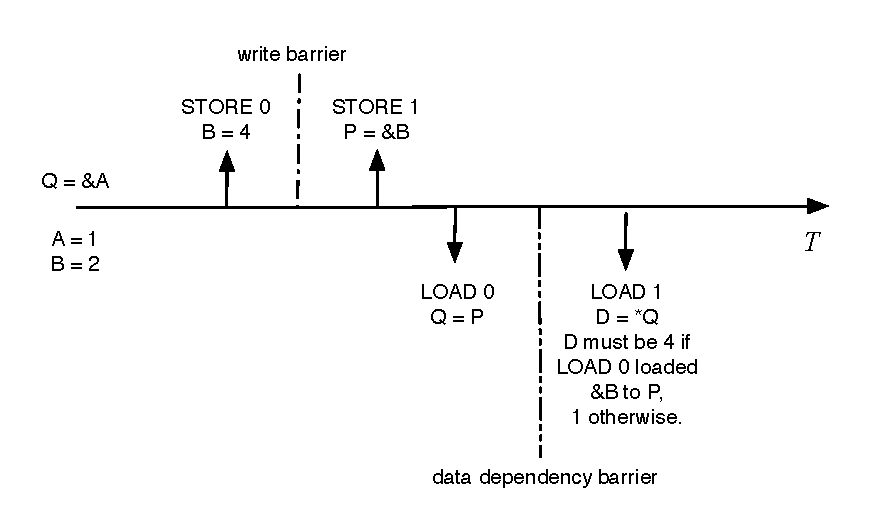
\includegraphics[scale=0.75]{fig/wmb_ddmb}
      \caption{写屏障及其配对的数据依赖屏障}
      \label{fig:ddmb}
    \end{figure}
    需要指出的是,
    如果没有那个data dependency barrier,
    在某些硬件体系结构(如:Alpha)上,
    完全可能发生Q = \&B但是D = 2这样的结果。
    导致这一看似违反因果律的一种可能原因是:
    P被读入奇数行的cache line而B被读入偶数行的cache line中,
    并且偶数行的cache line过于繁忙,
    于是P已经被更新但读取的B仍然是未被更新的cache值。
  \item {\em 读屏障}:
    读屏障保证了对系统的其它组件而言,
    屏障之前的读指令(LOAD)总是在在屏障之后的读指令之前被观察到。
    读屏障隐含了数据依赖屏障。
    同样地读屏障并不影响任何的写内存指令。
    通常写屏障之前的写入与读屏障或数据依赖屏障之后的读取相对应。
  \item {\em 通用屏障}:
    就是读写屏障,
    所有的读和写被屏障部分地有序化。
  \item {\em 半透屏障}:
    LOCK保证其后的访存操作不会出现在锁之前,
    同时UNLOCK保证之前的访存操作不会漏到其后,
    硬件必须保证这一半透屏障特性,
    否则同步就无从谈起了。
\end{itemize}

引起访存乱序还可能源自于编译器,
很多时候编译器会将它认为无依赖关系的指令重排实现优化,
如果希望某部分代码编译后指令一定要出现在另外一部分之前,
可以使用barrier()函数。

内存屏障一个重要场景是外设的MMIO实现。
外设的地址空间(端口,寄存器,内存)可以有两种方式访问,
一种称为{\em I/O Mapped},
另一种称为{\em Memory Mapped},
前一种方式使用\ins{in}/\ins{out}指令来访问外设地址空间,
后一种方式将外设地址空间映射到虚拟地址空间中,
一般建议用\ins{readb/w/l}或\ins{writeb/w/l}指令访问,
称为MMIO,
但是某些平台支持直接用指针访问I/O内存映射,
这种情况就必须适当使用内存屏障,
因为无论是CPU还是编译器都不知道外设地址空间到虚拟地址空间映射的逻辑。

\subsection{零拷贝}
假设一个简单场景,
用户进程调用read将数据读入一个用户态缓冲区,
而后将其通过write写入一个socket发送出去。
这个简单的应用实际上在内核空间导致了四次数据拷贝。
\begin{enumerate}
  \item DMA引擎将磁盘数据拷贝到内核缓冲区(假设数据不在page cache中)
  \item 接收到的数据被从内核缓冲区拷贝到read系统调用指定的用户态缓冲区中
  \item write系统调用把用户态缓冲区中数据拷贝到内核socket缓冲区
  \item 网卡的DMA引擎将内核的socket缓冲区中数据拷贝发送
\end{enumerate}
以上四个拷贝中的多数是可以通过某些硬件软件手段避免。

第一个可以想到的使用mmap替代read,
也就是将内核缓冲区映射到用户的虚拟地址空间中,
于是以上的第2个拷贝操作可以避免。
使用mmap的一个问题是,
当write过程中如果有另外一个进程把文件截断({\em truncate}),
写进程将收到一个SIGBUS信号。
显然在用户中代码简单地忽略SIGBUS信号绝对不可行,
一个正确的做法是在mmap之前先使用fcntl对该文件上一个租约({\em lease})锁,
当有其它进程试图截断该文件时,
本进程会收到一个RT\_SIGNAL\_LEASE信号,
其中RT代表real time。
进程的写操作被中断,
但是该写操作的errno为success,
返回已经写入的字节数。
而后进程被SIGBUS杀死。

自2.1版本起,
Linux内核提供sendfile系统调用,
其作用类似于上述mmap+write方案,
可以减少一次从内核缓冲区向用户态缓冲区的拷贝。
当有其它进程试图截断正在访问的文件时,
返回已处理的数据字节数并将errno设为成功,
不同的是,
系统仅发送RT\_SIGNAL\_LEASE而不发送SIGBUS。

需要更进一步提高效率,
从文件系统缓冲区向socket缓冲区的拷贝需要想办法消除。
这就需要硬件支持scatter/gather I/O的功能,
如本例中,
如果网卡的发送缓冲区可以是分散的内存位置,
而且网卡可以通过一次DMA操作即可将这分散的数据整合起来发送,
那么自文件系统缓冲区向socket缓冲区的那一次拷贝可以消除。
从内核2.4开始,
socket缓冲区被修改以支持此硬件功能,
简而言之就是传给硬件(DMA引擎)的参数不再是传统的地址+长度,
而是一个包含多个(可以不连续)的缓冲区的向量({\em vector}),
从而实现真正的CPU/OS层面上的``零拷贝''。

\subsection{访问用户空间地址}
编写内核模块代码过程,
当需要访问用户空间地址时必须使用%
\verb|copy_from_user|、
\verb|copy_to_user|、
\verb|get_user|、
以及\verb|put_user|系列函数完成,
不允许直接使用指针。

理论上说内核代码可以直接通过指针来访问用户地址空间中内容,
实际上在Linux下这样做也偶尔行得通,
但更多时候会导致内核或应用程序崩溃。
这是Linux内核基于一些简单原则所做的设计决定,
并非因为有不可逾越的技术障碍。

{\color{red}
In theory it's possible to access to the user space address
directly via a user land pointer,
and occasionally it works,
but most of the time this triggers a kernel oops.
Practically we use a serial of functions for user land address access,
for example,
\verb|copy_from_user|,
\verb|copy_to_user|,
\verb|get_user|,
\verb|put_user|,
etc.}

首先一个原则是内核态一般不允许触发缺页异常,
除了以下两个特例,
包括:
\begin{itemize}
  \item 缺页地址落在内核\verb|vmalloc|区
  \item 缺页地址位于用户地址空间,
  并且引发异常的代码位于\verb|fixup|段中
\end{itemize}
其它情况将引发{\em kernel oops},
并且内核将发送\verb|SIGKILL|杀死用户进程。
细节详见\verb|do_page_fault|函数。

\verb|fixup|文本段专门为了处理内核代码访问用户空间地址而设立。
所有需要访问用户空间的代码(大多是系统调用)使用统一的接口,
接口实现都放置({\em relocate})在\verb|fixup|文本段内,
称为{\em exception tables},
\verb|do_page_fault|调用\verb|search_exception_tables|搜索触发缺页的指令。

另外值得一提的是\verb|vmalloc|区的所有页映射已经建立,
为什么还可能触发缺页?
原因是\verb|vmalloc|区的映射建立的是一个内核主页表
(即所有进程的内核空间模板),
具体到某个进程,
映射可能并未建立,
所以这种异常发生之后,
内核调用\verb|vmalloc_fault|拷贝内核主页表给该进程。

\subsection{下划线函数名前缀}
历史上,
单下划线前缀被用于声明某些本应是内部私有,
但最终出于某些技术原因为外不可见的函数。
Linux应该也延续了这一传统。

Linux内核种有些函数以双下划线为前缀示意直接调用该函数要谨慎,
因为它们仅完成核心功能,
不执行参数校验、互斥等重要过程。
如果可能尽量使用不带双下划线的``安全''接口。

\subsection{常用宏定义}
\begin{itemize}
  \item {\tt offsetof}:取一个结构中某个域在该结构的偏移位置,
    当不能使用编译器提供的功能时,
    使用一个小技巧用宏实现:
    \inputclisting{src/offsetof.c}
                  {offsetof macro}{offsetof}
    %\lstinputlisting[language={C},%
    %                 caption={offsetof macro in C},%
    %                 label={lst:offsetof}]%
    %  {#define offsetof(TYPE, MEMBER) ((size\_t) \&((TYPE *)0)->MEMBER)}
  \item {\tt container\_of}:已知域的地址,求包含其域的结构地址:
    \inputclisting{src/container_of.c}
                  {container\_of macro}{cof}
  \item {\tt min(x, y)}:返回x和y中较小者,
    一个粗糙的宏定义如下,
    这个宏定义存在于无数的程序中,
    包括一些驱动程序,
    \newpage
    \inputclisting{src/wrong_min.c}
                  {naive min macro}{wmin}
    参数带着括号使用,
    这个宏定义依然是错的,
    原因在于该宏在程序执行时某个参数将被访问两次,
    于是象min(x++, y++)这样的调用将导致或者是x或者是y被自加两次。
    解决方法是使用gcc的\verb|({...})|扩展,
    在代码块内定义临时变量来存放参数,
    返回临时变量中较小的那一个:
    \inputclisting{src/min.c}
                  {correct min macro}{min}
    有意思的地方在于那个永不为真的地址比较,
    比较是为了在编译阶段就能察觉传入参数类型不一致,
    由于该比较对外界毫无影响,
    编译器将发出``has no effect''警告,
    加(void)的目的就是消除该警告,
    事实上该语句将不会被编译为任何指令。
    通常需要返回值的宏考虑使用\verb|{...}|扩展。
  \item {\tt do\{...\}while(0)},
    在Linux内核中多数包含多条语句的宏定义采用do\{...\}while(0)
    的形式,而不是简单地将多条语句包含在一对花括号中。
    首先考虑不采用包含在一对花括号中的情况,
    多条语句顺序在宏中出现,
    考虑如下代码
    \inputclisting{src/bad_macro0.c}
                  {bad macro0}{bm0}
    调用宏的语句出现在if/else场景中,
    宏展开后statement1;出现在else之前,
    导致C语法错误。
    将多条语句包含在一对花括号中可以解决问题,
    但是调用宏的语句不能以分号结束,
    如下代码正确但是有点丑陋,
    C语句不以分号结束不符合普遍编程习惯:
    \inputclisting{src/bad_macro1.c}
                  {bad macro1}{bm1}
    解决方法就是内核所使用的do\{...\}while(0)小技巧:
    \inputclisting{src/good_macro.c}
                  {good macro}{gm}
\end{itemize}

\subsection{Buddy System}
无控制的任意尺寸页帧分配和释放最终将%
导致内存中布满了分隔的大量小尺寸可用页帧,
从数量上虽然有足够可用内存,
却没有一块连续的大尺寸页帧满足分配请求,
这就是所谓外部碎片。
{\em Buddy System}设计用于有效减少外部碎片。

Linux下Buddy System的思路如下:
\begin{enumerate}
  \item 将所有页帧归为不同的组,
    每个组包含连续也帧数是2的$n$幂,
    指数$n$取值自0至10,
    相同指数的页帧用链表组织,
    11个链表头保存在zone的mem\_map数组域中,
    指数即作为该数组的索引。
  \item 当试图分配尺寸为2的m次幂个页帧时,
    首先查找指数为m的组,
    如果有可用页帧组则返回该组,
    否则查找指数加一的组,
    关键的是,
    当实际分配的页帧组指数小于从中分配的页帧组指数是,
    该页帧组剩余的页帧组要被相应插入到指数小的链表中;
  \item 释放一组页帧时,
    如果该组有一个“伙伴”,
    则和其伙伴合并为一个指数高一级的组
    继续找伙伴合并过程直至无法找到合适的伙伴。
    两个页帧组可以成为伙伴必须满足:
    \begin{enumerate}
      \item 两个组相邻
      \item 两个组有相同的尺寸,假设为$b$
      \item 两个组如果合并为一个大组,
        大组的第一个页的起始地址必须为$2 \times b \times 2^{12}$的整数倍,
        换句话说就是合并后的大组首地址按$2b$页方式对齐,
        要找一个组和其伙伴合并后的大组的首地址用异或实现:
        $buddy\_idx = page\_idx \XOR (1 <\!<\! b)$,
        异或实际效果是switch了一个地址的第$b$位,
        亦即如果该位原来为0,
        结果是比该组地址高$b \times 2^{12}$的地址,
        否则是比该组地址低$b \times 2^{12}$的地址,
        这就保证了合并后的大组首地址按$2b$页对齐
    \end{enumerate}

\end{enumerate}

\subsection{Slab Allocator}
\begin{figure}[!ht]
\centering
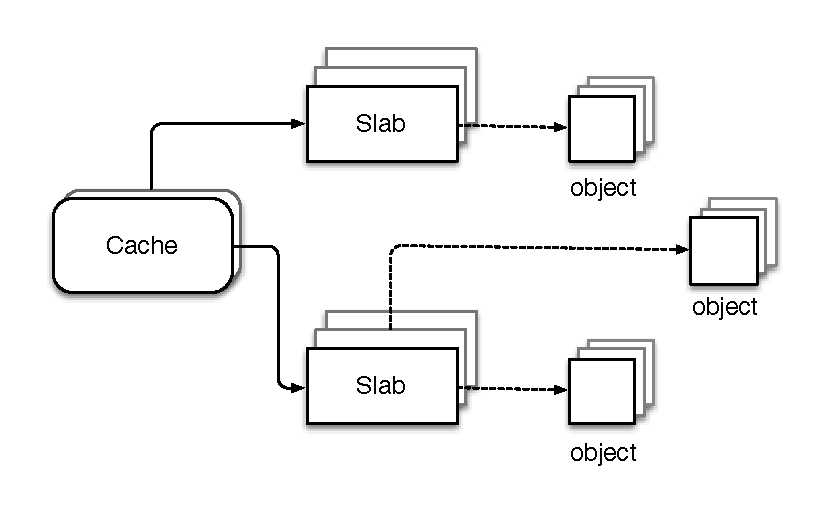
\includegraphics[scale=0.8]{fig/slab}
\caption{Cache、Slab,及对象}
\label{fig:slab}
\end{figure}

{\em Slab Allocator}解决如下问题:
\begin{itemize}
  \item 统一管理所谓{\em free list}缓存,
    对于频繁分配释放的数据结构,
    一般程序员会一次性分配大块内存用作缓存,
    即数据结构从缓存中分配,
    释放数据结构也不立即交还系统(譬如Buddy System)而是放入free list中%
    以备随时再次分配。
    这种free list方案带来的问题是,
    内核无法统一管理,
    于是干脆提供一个为所有模块服务的缓存机制。

  \item 内部碎片,
    由于内核分配以页为单位,
    如果不有效管理利用,
    一个页内会有无用空间,积少成多数量也很可观,
    这就是所谓内部碎片问题。

  \item 内核的开发人员可以在slab这一层加入一些高级的优化策略,
    譬如,上色降低相同类型的缓存被放置于同一条缓存线上({\em cache line})。
\end{itemize}

如图\,\ref{fig:slab}\,所示:
一个数据结构占据一段连续的内存,
称为一个“对象”,
用于存放一组相同数据类型的对象称为“slab”,
一个slab可以占据一个或多个连续的物理页帧,
所有的slab组成该类型的“cache”。

如图\,\ref{fig:slabc}\,所示,
颜色属性尽量将一个slab和另一个同类型slab对象的起始地址错开,
降低它们落入同一条缓存线的几率。

\begin{figure}[!ht]
\centering
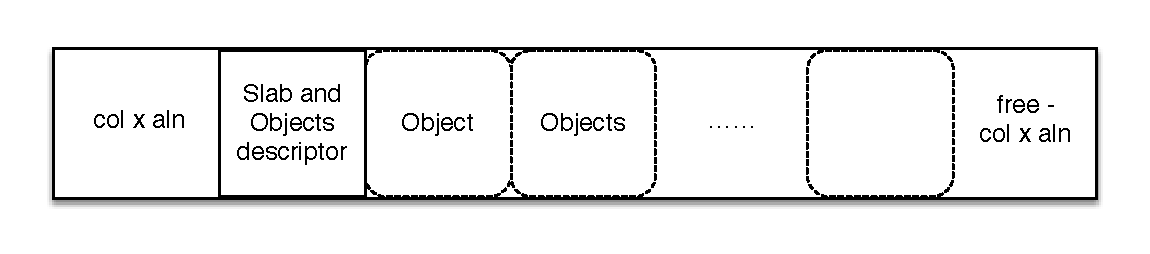
\includegraphics[scale=0.75]{fig/slab_color}
\caption{Slab Coloring}
\label{fig:slabc}
\end{figure}

\section{内核崩溃诊断}

\end{document}
